\documentclass{article}

% Language setting
% Replace `english' with e.g. `spanish' to change the document language
\usepackage[spanish, es-nodecimaldot]{babel}
\usepackage[most]{tcolorbox}

% Set page size and margins
% Replace `letterpaper' with `a4paper' for UK/EU standard size
\usepackage[letterpaper,top=2cm,bottom=2cm,left=3cm,right=3cm,marginparwidth=1.75cm]{geometry}

% Useful packages
\usepackage{amsmath}
\usepackage{graphicx}
%\usepackage{subfigure}
\usepackage{caption}
\usepackage{subcaption}
\usepackage[colorlinks=true, allcolors=blue]{hyperref}

\newtcolorbox[auto counter, number within=section]{exercise}[1][]{
    colback=blue!5!white,
    colframe=blue!75!black,
    fonttitle=\bfseries,
    title=Ejercicio \thetcbcounter,
    #1 % Allows you to add custom options locally (like labels)
}




\title{Reinforcement learning I}
\author{Arturo Gil y Juan José Cabrera}

\begin{document}
\maketitle

\section{Introducción}
La mayor parte de los conceptos vistos hasta el momento en la asignatura se pueden clasificar como algoritmos de aprendizaje supervisado. Dentro de este tipo de aprendizaje consideramos algoritmos a los que se le proporciona un conjunto de datos de entrenamiento etiquetados. El rol del algoritmo es encontrar una función que permita hallar una mapeo lo más aproximado posible entre las entradas y las salidas proporcionadas. En el ámbito del aprendizaje por refuerzo (\emph{reinforcement learning}) se plantea un problema que difiere significativamente del anterior: se desea que un agente alcance algún grado de aprendizaje o inteligencia sin utilizar datos de entrenamiento etiquetados. Los únicos datos disponibles son aquellos que genera el agente mientras interactúa con el entorno. A continuación indicamos algunos ejemplos de aprendizaje con refuerzo (\textit{reinforcement learning}):
\begin{itemize}
    \item Un robot en un laberinto (figura \ref{fig:robot_in_a_maze}): asuma que tenemos un robot en un laberinto. Se trata de un robot omnidireccional. Así pues, en cada momento el robot puede moverse en 4 direcciones (izquierda, derecha, arriba o abajo). Consideramos que en todo momento podemos conocer la posición del robot en el laberinto. El objetivo del problema es que el robot sea capaz de encontrar el camino óptimo que le lleve a la salida, cuando el robot parte desde diferentes puntos de inicio. Así pues, el aprendizaje consiste en que el robot se forme una especie de mapa mental que le permita tomar la mejor acción (moverse a la izquierda, derecha, arriba abajo) en cada punto del mapa y que estas acciones lo lleven siempre a la salida.
    \item Imaginemos ahora que tenemos un robot bípedo como el mostrado en la figura \ref{fig:robot_bipedo}. En este caso, nos gustaría poder programar al robot para que pudiera andar. Imaginemos también que tenemos un modelo dinámico que nos permite simular el sistema en el ordenador (figura \ref{fig:robot_bipedo_gymnasium}). Finalmente, sabemos que la marcha bípeda es extremadamente compleja, pues todas las variables del sistema están acopladas. Igualmente, las ecuaciones dinámicas del sistema son altamente no lineales y están acopladas: cuando se aplica un par a una articulación (mediante un motor) también se generan reacciones de fuerzas y pares en otras articulaciones. En este caso, en vez de plantear un control de las variables articulares, ¿por qué no utilizamos un algoritmo de aprendizaje que use el simulador y pruebe diferentes soluciones para que el agente pueda caminar? Durante la simulación, cada vez que el robot realice un movimiento que le permita avanzar, recibirá un premio. Por contra, cada vez que el robot se caiga al suelo, se castigará.
\end{itemize}

Merece la pena decir aquí que, como en casi todos los ámbitos del conocimiento, existen soluciones alternativas. Así pues, en el primero de los problemas planteados, un ingeniero especialista en el ámbito de la robótica móvil nos diría que también se podría plantear la construcción de un mapa de ocupación con alguna técnica de \emph{mapping} o \emph{SLAM} para después utilizar el algoritmo $A^*$ y planificar una ruta óptima (este algoritmo se ha estudiado en una práctica anterior). En el caso de los robots caminantes, también hay otras formas de plantear el problema: típicamente, un ingeniero definiría con cuidado el \emph{gait} de cada articulación y después intentaría optimizarlo en base a los parámetros dinámicos del robot.

\section{Objetivos} 

En esta práctica se recordarán algunos conceptos de aprendizaje por refuerzo y, en concreto, del algoritmo conocido como Q-learning tabular. Seguidamente, se verán algunos ejemplos de Q-learning usando la librería Gymnasium para python. \textbf{El estudiante experimentará de diferentes formas con estos entornos y observará qué ocurre con el aprendizaje cuando se cambian los hiperparámetros del algoritmo.}

\begin{figure}
    \centering
    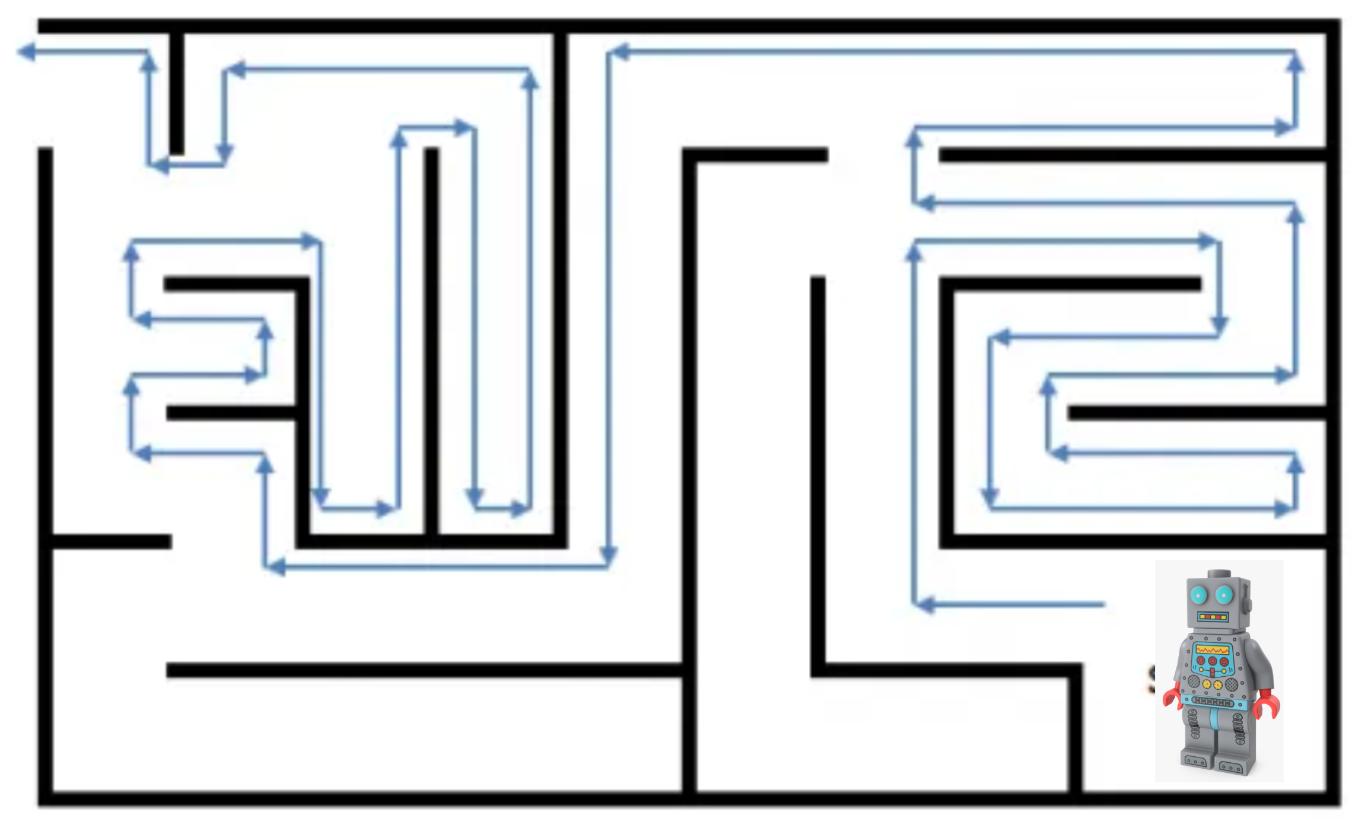
\includegraphics[width=0.7\linewidth]{figures/maze.png}
    \caption{Un robot en un laberinto}
    \label{fig:robot_in_a_maze}
\end{figure}

\begin{figure}
    \centering
    \begin{subfigure}{0.25\textwidth}
        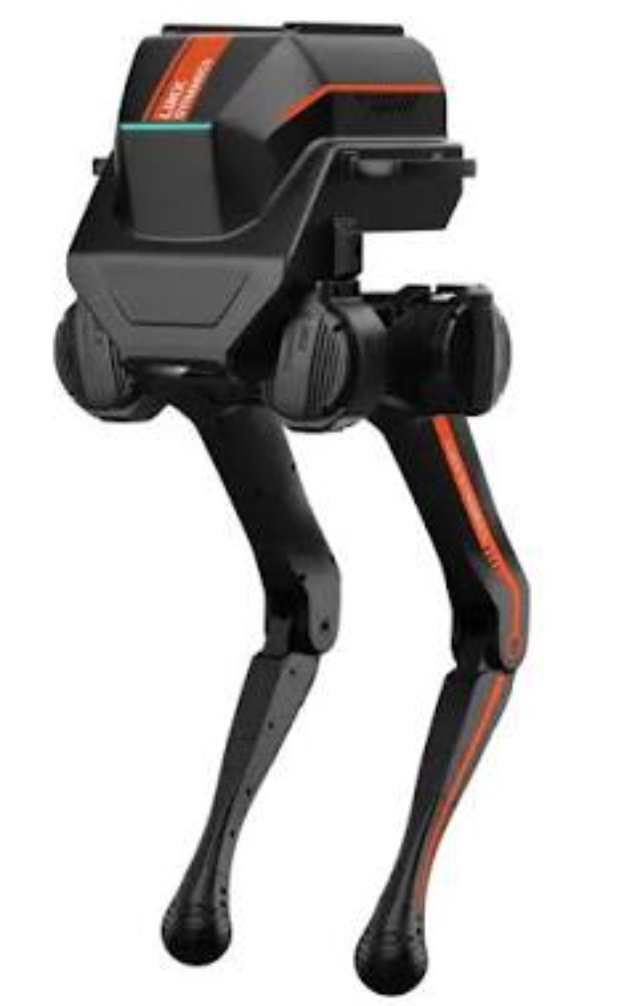
\includegraphics[width=\linewidth]{figures/bipedal_tron.png}
        \caption{Un robot bípedo.}
        \label{fig:robot_bipedo}
    \end{subfigure}
    \hfill
    \begin{subfigure}{0.6\textwidth}
        
\includegraphics[width=\linewidth]{figures/bipedal_gymnasium.png}
         \caption{Un robot bípedo simulado en Gymnasium.}
        \label{fig:robot_bipedo_gymnasium}
    \end{subfigure}
    \caption{Un robot bípedo real (arriba) y simulado (abajo).}
    \label{fig:robots_bipedos}
\end{figure}


\section{El repositorio de prácticas y Gymnasium}
Se os proporciona un repositorio de Github con algunos scripts que usan el algoritmo Q-learning y están basados en la librería Gymnasium (\url{https://gymnasium.farama.org/}). Se trata de una librería para python que incluye una serie de entornos y agentes y es especialmente adecuada para probar y desarrollar algoritmos de aprendizaje por refuerzo. Si quieres observar estos entornos, visita \url{https://gymnasium.farama.org/environments/classic_control/}, por ejemplo para ver los ejemplos de reinforcement learning para problemas clásicos de control (el péndulo invertido, cart-pole, etc...). La librería es realmente interesante y permite, entre otras cosas, entrenar a un agente para que sea capaz de jugar a cualquiera de los 106 juegos de la consola Atari 2600 (comercializada en 1977).


\section{Algunos conceptos de \textit{reinforcement learning}}

\subsection{Q-learning}
El algoritmo Q-learning es uno de los más famosos en el ámbito del aprendizaje por refuerzo. Se trata un algoritmo que no precisa de modelos del entorno ni del agente. El algoritmo busca la estimación de una tabla Q donde cada fila representa un estado $s$ y las columnas representan las posibles acciones $a$ que puede realizar el agente en cada estado. En cada celda de la tabla se almacena un valor $Q(s, a)$ que estima la recompensa futura (sobre todos los estados futuros hasta el final del episodio) de tomar la acción $a$ cuando el agente se encuentra en el estado $s$. La tabla se calcula durante el entrenamiento usando la ecuación de Bellman. Durante la fase de funcionamiento (test), el agente ejecuta la acción $a$ para la cual el valor en la tabla es máximo.
También consideramos que en un momento determinado de tiempo $t$, el estado del agente y del entorno se puede describir mediante $s_t \in S$ (es decir, un estado $s_t$ dentro del conjunto de posibles estados que describen al agente y al entorno). Asumimos que en ese mismo instante el agente decide realizar una acción $a_t \in A$. Contamos con un modelo de transición de estados (también llamado un modelo de movimiento). Este modelo se representa de dos formas diferentes:
\begin{itemize}
    \item En el caso más sencillo: $s_{t+1}=\delta(s_t, a_t)$. Dado que el robot se encuentra en $s_t$, si se ejecuta la acción $a_t$ entonces el estado cambiará a ser $s_{t+1}$. En el ejemplo inicial del laberinto, el robot se moverá a la siguiente posición, dependiendo de la acción $a_t$ que se realice (arriba, abajo, izquierda o derecha) y, además, dependiendo de si hay una pared en el laberinto o si el espacio está libre. Esta situación contempla el caso en el que el modelo de movimiento del agente es determinista.
    \item En el caso más general, hablaremos de un modelo de transición de estado probabilístico. Estos modelos son instancias de MDP (\emph{Markov Decision Processes}) y se representan mediante una función de probabilidad condicionada
    $P(s_{t+1}|s_t, a_t)$. Es decir, dado que el agente y entorno se encuentran en $s_t$ y se ejecuta la acción $a_t$, podemos establecer una función de probabilidad sobre el estado futuro $s_{t+1}$.
\end{itemize} 

\subsection{Estados y acciones}
En esta práctica trabajaremos con el caso en el que el estado y las acciones se pueden describir de forma discreta. En una práctica posterior (\textit{reinforcement learning II}) trabajaremos con el caso en el que el estado es continuo y las acciones discretas. El caso más complejo es aquél en el que tanto el estado como las acciones son continuas. Ejemplos:
\begin{itemize}
    \item Estado y acciones discretas: \textit{Taxi} y \textit{Cliff Walking}.
    \item Estado continuo y acciones discretas: \textit{Lunar Lander}.
    \item Estado y acciones continuas: \textit{Bipedal Walker}.
\end{itemize}


\subsection{Etapas y episodios}
Una etapa (paso o step) del algoritmo comprende el caso en el que el agente se encuentra en un estado $s_t$, realiza una acción $a_t$ que la conduce a otro estado $s_{t+1}$ (y recibe una recompensa $r_{t}$).

Un episodio incluye un número variable de pasos. En un episodio existe un inicio y un final: generalmente el agente debe ser capaz de cumplir una misión. En algunos procesos podemos establecer de forma natural cuándo se inicia y se finaliza la misión. En el caso del robot en el laberinto, el episodio comienza con el robot en la casilla inicial y finaliza cuando el robot llega a la casilla de salida (o bien cuando se ha superado un número máximo de pasos). Realizada la última acción por el robot, la misión finaliza y, por tanto, podemos decir que el episodio acaba.

En otras situaciones, como en el caso en el que se quiere controlar un proceso continuo, el concepto de episodio no es adecuado, pues el control debe funcionar \textit{ad eternum}. %Normalmente, un episodio durará una serie de pasos máximos (por ejemplo, 200 pasos).
Será importante que el estado inicial $s_0$ varíe en el comienzo de cada episodio. Este hecho es fundamental para que el agente aprenda de una forma general.

\subsection{Entrenamiento}

El objetivo del entrenamiento es maximizar la suma de las recompensas de cada episodio. Esto supone que las recompensas deben estar bien definidas. Según se definan las recompensas, así será el resultado final del aprendizaje.  Así pues, los pesos de las recompensas deben ser elegidos cuidadosamente y con rigor para que se produzca un correcto aprendizaje. En los casos de aprendizaje en los que se desea que un robot camine, se premia con +1 cada vez que el robot avanza en la dirección deseada y con -10, por ejemplo, cuando el robot pierde el equilibrio y se cae.



\subsection{Train y test}
En el paradigma del aprendizaje con refuerzo, se plantean generalmente dos fases separadas: 
\begin{itemize}
    \item Entrenamiento (\textit{train}): se plantea inicialmente una etapa en la que el agente se entrena, obteniendo conocimiento sobre el entorno, según realiza acciones y obtiene recompensas.
    
\item Prueba, funcionamiento o \textit{test}: se plantea, después, otra etapa en la que se prueba el algoritmo con el objetivo de medir sus capacidades.
\end{itemize}

 En ambas etapas nos interesa medir el comportamiento del agente para evaluar sus conocimientos. También es frecuente que tengamos que variar los parámetros del algoritmo para mejorar su aprendizaje. Aquí se apunta alguna información que debe ser almacenada en cada episodio para observar el aprendizaje:
 \begin{itemize}
     \item Suma de recompensas en cada episodio.
     \item Histograma de los estados visitados en todos los episodios. Para comprobar si el agente ha podido visitar todos los estados posibles y, en cada uno de ellos, ha podido probar todas las acciones disponibles.

     \item Imagen de la tabla Q. Permite visualizar rápidamente las acciones para diferentes estados discretos.
 \end{itemize}




\subsection{Exploitation, exploration and reward}
Definimos a continuación los conceptos de explotación, exploración y recompensa (\textit{exploitation, exploration and reward}):
\begin{itemize}
    \item \textit{Exploitation}: hace referencia al cálculo de una acción a realizar cuando se hace uso del conocimiento actual sobre la acción que produce una mejor recompensa futura. En el algoritmo Q-learning, el conocimiento se almacena en la tabla Q. 
    
    \item \textit{Exploration}: se habla de exploración cuando el agente toma decisiones aleatorias. Al tomar acciones aleatorias, el agente puede llegar a estados que permiten mejorar el conocimiento que tenemos sobre las recompensas y el entorno. El concepto de exploración responde a la pregunta ¿qué pasa si estando en este estado llevo a cabo una acción aleatoria $a_t$, obtendré una recompensa futura mayor?
\end{itemize}

\textbf{En general, explotar el conocimiento que tenemos permite maximizar la recompensa actual, pero la exploración permite probar nuevas formas de resolver el problema que podrían producir una recompensa total futura mayor.}


%Ahora mismo es mejor que aprendáis a resolver este problema poco a poco, os llevará más tiempo y esfuerzo ahora, pero ahorraréis tiempo en el futuro. Si le preguntáis a la IA ahora, os dará una solución rápida pero, seguramente, no aprenderéis, y a la larga os costará más aplicar esta solución a un problema más complejo.

En un único paso del algoritmo no es posible explorar y explotar al mismo tiempo, pues únicamente podemos aplicar la acción una vez y, a continuación, el agente pasará a estar en un estado diferente. Así pues, en ocasiones se habla del conflicto entre la exploración y la explotación del conocimiento que se tiene en un determinado momento: el agente se podría plantear en cada momento, ¿qué hago?, ¿explorar o explotar el conocimiento que he recabado hasta ahora? Así pues, en un momento determinado del ciclo de aprendizaje, nos podríamos preguntar, ¿cómo de seguros estamos de que tenemos un conocimiento correcto sobre la tabla $Q(s,a)$. Por ejemplo, imaginemos que el agente ha llegado a un estado $s_t=8$ y consulta la tabla $Q(s,a)$ donde se obtiene una acción $a_t$=GO RIGHT. Después de realizar esa acción, el agente obtiene una recompensa $r_t=1$. Imaginemos que ahora estamos en un episodio diferente y hemos llegado al mismo estado $s_t=8$ de nuevo. Nos preguntamos ahora si a) debemos repetir la acción anterior y asegurar una recompensa inmediata de 1 punto o, b) elegir otra acción diferente, esperando que esto dé lugar, al final del episodio, una recompensa final mayor.

La forma más académica de resolver el dilema entre la exploración y la explotación es plantear qué incertidumbre tenemos sobre la matriz Q. Imaginemos que el agente que está tomando decisiones es un estadístico. Podría evaluar las acciones que se habían tomado con anterioridad y calcular la incertidumbre con la que se conoce esta información. Cuando la incertidumbre sobre las estimaciones sea  baja, el estadístico debería decidir que ya no es necesario más acciones exploratorias y se debe usar únicamente las acciones que indique la tabla $Q$.

\subsection{Algoritmo greedy y epsilon greedy}
En esta práctica se plantea una forma sencilla de articular la exploración y la explotación. Esta forma de proceder se denomina $\epsilon$-\textit{greedy} (epsilon \textit{greedy}). Esta política funciona de la siguiente manera: se inicializa $\epsilon=1$ y se programa una función que decrece con el paso de los episodios de la siguiente manera:
\begin{verbatim}
    for episode in episodes:
        environment.reset()
        epsilon = 1.0
        while True
            # running episode i
            p=normrnd()
            if p < epsilon:
                exploration: random action
            else
                exploitation: computed action
            s_{t+1} = environment.step(action)
        epsilon = delta*epsilon
\end{verbatim}

Así pues, con probabilidad $\epsilon$ se explora y con probabilidad $1-\epsilon$ se explota el conocimiento. El valor de $\epsilon$ se va reduciendo en cada episodio, pues es preferible tomar acciones aleatorias durante los primeros episodios del aprendizaje y refinar el conocimiento durante los episodios finales. Esta estrategia se denomina $\epsilon$-greedy con decaimiento. La estrategia consiste en reducir $\epsilon$ según avanza la simulación al multiplicarlo por un factor $\delta$:
\begin{equation}
    \epsilon_{t+1}= \epsilon_{t}\cdot\delta
\end{equation}
Esta operación se hace, bien durante cada paso de la simulación o bien en cada episodio. En esta práctica, reduciremos $\epsilon$ en cada episodio. Además, se fija un valor mínimo $\epsilon_{min}$:
\begin{equation}
    \epsilon_{t+1}= \max(\epsilon_{min}, \epsilon_{t}\cdot\delta)
\end{equation}

Generalmente, se calcula $\delta$ para que $\epsilon$ vaya de su valor máximo a su valor mínimo en una fracción de los episodios de entrenamiento. Es típico calcular el factor de decaimiento $\delta$ para que pase de $\epsilon_{max}$ a $\epsilon_{min}$ en un 25\% del total de episodios de entrenamiento. Así, si por ejemplo, el total de episodios de entrenamiento es $N=1000$, entonces $N_{target}=N\cdot 0,25=250$ y calculamos:

$$\delta = \left(\frac{\epsilon_{\text{min}}}{\epsilon_{\text{max}}} \right)^{\frac{1}{N_{target}}}$$

Por ejemplo:
\begin{itemize}
    \item $N=1000$.
    \item $N_{target}=250$.
    \item $\epsilon_{max}=1.0$ (valor inicial).
    \item $\epsilon_{min}=0.01$ (valor final).
    \item $\delta=0.98174$.
\end{itemize}
Es fácil comprobar que $\epsilon_{max}\cdot \delta^{250}\approx 0.01$. Se usan diferentes tipos de funciones para variar el valor de $\epsilon$ en función de los episodios. Se listan las más importantes:
\begin{itemize}
    \item Geométrica: $\epsilon_{t+1} = \max(\epsilon_{\min}, \epsilon_t \cdot \delta)$, con $0 < \delta < 1$. 
    \item Exponencial: 
    \item Lineal: $\epsilon_t = \max(\epsilon_{\min}, \epsilon_0 - \delta \cdot t)$, siendo $\delta$ es un paso fijo. 
    \item Tiempo inverso: $\epsilon_t = \frac{\epsilon_0}{1 + \delta \cdot t}$ 
\end{itemize}
%\textcolor{red}{JUANJO: no he metido la fórmula de $$\epsilon_t = \epsilon_{min}+(\epsilon_{max}-\epsilon_{min})e^{-\delta t}$$ porque la forma recursiva no es posible obtenerla exactamente. La forma aproximada: $$\epsilon_t=\epsilon_{max}e^{-\delta t}$$, al final, da la misma curva que la geométrica}

Se proporciona al estudiante una clase base \texttt{EpsilonGreedy} y tres clases derivadas (\texttt{EpsilonGreedyGeom}, \texttt{EpsilonGreedyLinear} y \texttt{EpsilonGreedyInverseTime}) que implementan cada uno de los anteriores protocolos para $\epsilon$. En la figura X.X se muestra el resultado de ejecutar los objetos de las clases derivadas (\texttt{EpsilonGreedyGeom}, \texttt{EpsilonGreedyLinear} y \texttt{EpsilonGreedyInverseTime}) con $N=1000$, $N_{target}=250$, $\epsilon_{max}=1.0$ y $\epsilon_{min}=0.01$.


\textbf{NOTA}: En los problemas que resolveremos en estas prácticas usaremos la regla del 25/75 (frecuente en el área del aprendizaje con refuerzo   \cite{sutton2018reinforcement}). Así, si pensamos entrenar durante 1000 episodios, usaremos 250 a explorar (con alta probabilidad) y 750 para refinar la solución. Estos porcentajes, claro está, se deben variar para adaptarse al problema en cuestión: de esta adaptación dependerá en gran medida el resultado del entrenamiento.
%Id est: durante los primeros episodios se explora más (en busca de nuevo conocimiento) y durante los últimos se explota más el conocimiento que se posee. Esta estrategia se denomina método epsilon-greedy de exploración-explotación.


\begin{figure}
    \centering
    \begin{subfigure}{0.49\textwidth}
        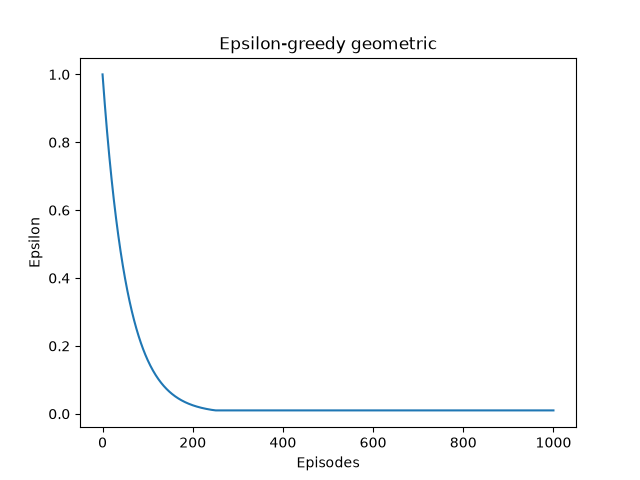
\includegraphics[width=\linewidth]{figures/epsilon_greedy_geometric.png}
        \caption{\texttt{EpsilonGreedyGeom}.}
        \label{fig:epsilon_greedy_geom}
    \end{subfigure}
    \hfill
    \begin{subfigure}{0.49\textwidth}
        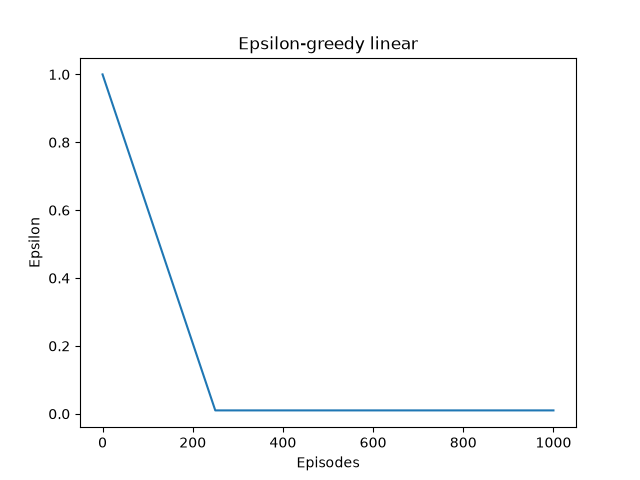
\includegraphics[width=\linewidth]{figures/epsilon_greedy_linear.png}
         \caption{\texttt{EpsilonGreedyLinear}.}
        \label{fig:epsilon_greedy_linear}
    \end{subfigure}
    \hfill
    \begin{subfigure}{0.49\textwidth}
        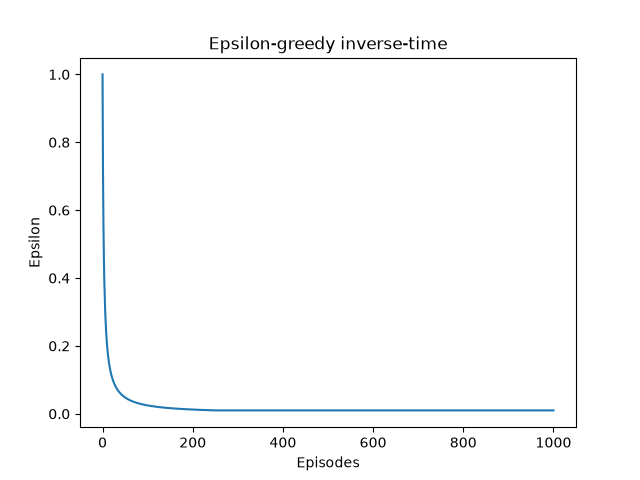
\includegraphics[width=\linewidth]{figures/epsilon_greedy_inverse_time.png}
         \caption{\texttt{EpsilonGreedyInverseTime}.}
        \label{fig:epsilon_greedy_inverse_time}
    \end{subfigure}
    \caption{Valores de $\epsilon$ por episodio para las diferentes clases \texttt{EpsilonGreedyGeom}, \texttt{EpsilonGreedyLinear} y \texttt{EpsilonGreedyInverseTime}.}
    \label{fig:epsilon_greedy}
\end{figure}




%\subsubsection{Actualización de Q (primera versión)}
%En esencia, la tabla $Q(s_t,a_t)=r_t$ se puede entender de la siguiente manera:
%\begin{itemize}
%    \item Dado un estado $s_t$.
%    \item Almacena un valor para cada una de las posibles acciones $a_t$ que puede ejecutar el agente en ese estado.
%    \item Sabemos que el agente elegirá la acción como: $a_t=argmax(Q(s_t, a_t)).
%\end{itemize}

%Se propone una actualización de la tabla Q en la que se hace:
%$$Q(s_t,a_t)=r_t$$

%\begin{exercise}
%    Complete la función \texttt{update\_q\_table} haciendo que:
    % $$Q(s_t,a_t)=r_t$$
%     Ejecute el algoritmo de \textit{train} varias veces y responda a las siguientes cuestiones:
%     \begin{itemize}
%         \item ¿El algoritmo consigue aprender?
%         \item ¿El agente consigue completar la misión en algún momento?
%     \end{itemize}
% \end{exercise}


% \subsubsection{¿Está aprendiendo el agente?}
% Efectivamente, es necesario saber qué esta pasando en cada episodio durante el entrenamiento. En caso contrario, vamos ``a ciegas''. En el futuro nos enfrentaremos a problemas más complejos y es vital que sepamos si se está produciendo algún tipo de aprendizaje, pues, en caso contrario, deberíamos parar el algoritmo de aprendizaje y volver a la fase de diseño. 
% \begin{exercise}
%     \begin{itemize}
%     \item Se propone que calcules la recompensa de cada episodio.
%     \item Se propone que plotees (o lo imprimas por pantalla) la tabla Q al final del aprendizaje para ver qué está pasando. 
% \end{itemize}
% \end{exercise}



% Según se ha podido comprobar, la actualización de la tabla Q anterior no es correcta. Así pues, la estrategia $Q(s_t, a_t)=r_t$ no produce buenos resultados. Debemos preguntarnos de nuevo: ¿qué representa $Q(s_t,a_t)$ en el problema? 
\subsection{Estimación de la tabla Q}
En el algoritmo Q-Learning, el valor de un elemento de la tabla $Q(s_t,a_t)$ representa una estimación de todas las recompensas futuras que se obtendrían hasta el final del episodio, al realizar la acción $a_t$ estando el agente en el estado $s_t$. %Así pues,  $Q(s_t,a_t)=r_t$ es \textbf{inadecuada}, pues está almacenando solamente la recompensa actual y no la suma de recompensas hasta el final.
Se plantea a continuación, una deducción sencilla de algunas expresiones que nos permiten estimar la tabla $Q$. Al final del apartado, llegaremos a la expresión de la ecuación de Bellman. 

Según se ha dicho, nos gustaría que $Q(s_t,a_t)$ guardara una estimación de las recompensas futuras que se obtendrían cuando el agente está $s_t$ y se toma la acción $a_t$, es decir:
$Q(s_t,a_t)=r_t + r_{t+1} + r_{t+2} + r_{t+3}$. Para ello, vamos a considerar que tenemos un entorno donde el número máximo de pasos es $T$ (como ocurre en la mayoría de entornos de Gymnasium). Así pues:
\begin{equation}\label{eq:estandar_sum_of_rewards}
Q(s_t,a_t) = \sum_{i=t}^{T} r_i= r_t +  r_{t+1}+ \ldots + r_T
\end{equation}
Suponga que en el instante siguiente $t+1$, el agente se ha movido hasta el estado $s_{t+1}$. El valor $Q(s_{t+1},a_{t+1})$ de la matriz Q también debería almacenar la suma de recompensas hasta el final del episodio:
\begin{equation}
Q(s_{t+1},a_{t+1}) = \sum_{i=t+1}^{T} r_i = r_{t+1} +r_{t+2} + \ldots + r_T     
\end{equation}

Podemos hacer: 
\begin{equation}
    Q(s_t,a_t) - Q(s_{t+1},a_{t+1}) = r_t
\end{equation}
Con lo que tenemos una primera forma de calcular un valor de la tabla Q:
\begin{equation*}
Q(s_t,a_t) = r_t + Q(s_{t+1},a_{t+1})   
\end{equation*}
Analizamos, seguidamente, esta expresión. Durante la simulación, en un instante determinado, conocemos que el agente está en $s_t$ y realiza la acción $a_t$, así pues, el elemento de la tabla a actualizar $Q(s_t , a_t)$ es fácil de identificar. Como consecuencia de la acción realizada, en ese mismo instante, el agente recibirá una recompensa $r_t$. El problema, ahora, consiste en sumar el término $Q(s_{t+1},a_{t+1})$. De este término, conocemos $s_{t+1}$. Dado $s_{t+1}$, tendremos diferentes valores de $Q(s_{t+1}, a_{t+1})$, para cada una de las posibles acciones $a_{t+1}$ que se pueden realizar en el instante siguiente. En consecuencia, ¿qué valor elegimos de $Q(s_{t+1},a_{t+1})$? La solución consiste en elegir el máximo de estos valores, pues el agente elegirá la acción que maximice las recompensas futuras. Así, se propone una \textbf{primera forma para estimar la tabla Q}:
\begin{equation*}
Q(s_t,a_t) = r_t + max_a(Q(s_{t+1},a))
\end{equation*}

Nótese que esta ecuación se debe ejecutar de forma repetida para poder llegar a una estimación final, pues inicialmente se desconocen los valores de la tabla Q. 

\subsection{\textit{Back-propagation}}
Nos volvemos a fijar en la ecuación para actualizar $Q$:
\begin{equation*}
Q(s_t,a_t) = r_t + max_a(Q(s_{t+1},a))
\end{equation*}
Debemos fijarnos en que se produce una propagación hacia atrás en el tiempo (de $t+1$ a $t$). Una forma de entender el funcionamiento básico del aprendizaje es esta: \textbf{``imaginemos que un estado futuro $s_{t+1}$ recibe una recompensa alta cuando consigue, por azar, la misión. Entonces el valor de $Q(s_t, a_t)$ se incrementará cuando $a_t$ lleve al agente al estado $s_{t+1}$''}. De forma recurrente, podemos pensar que en otra iteración del algoritmo se aumentará el valor de $Q(s_{t-1}, a_{t-1})$ cuando $a_{t-1}$ conduzca al agente a $s_{t}$. Vemos, por tanto, que debe existir una propagación hacia atrás desde los estados finales que están cerca de resolver el problema hasta los estados iniciales.



\subsubsection{El factor de descuento $\gamma$}
En algunos problemas, la suma de recompensas que se ha propuesto no resulta adecuada, pues la suma de recompensas pondera por igual los valores recibidos en el instante actual y los que se recibirán en el futuro (dentro de 100 pasos, por ejemplo). En la literatura es habitual modificar la suma de recompensas de la ecuación (\ref{eq:estandar_sum_of_rewards}) por la siguiente expresión:
\begin{equation}
Q(s_t,a_t) = r_t + \gamma r_{t+1}+ \gamma^2 r_{t+2} + \gamma^3r_{t+3} +  \ldots + \gamma^T r_T = \sum_{i=t}^{T} \gamma^{i-t}r_i
\end{equation}
Con este factor $0\leq\gamma\leq1$ se consigue que el agente pueda dar menos peso a las recompensas más alejadas del instante $t$ (los pasos siguientes). Igual que hicimos antes:
\begin{eqnarray*}
Q(s_t,a_t) &=& r_t + \gamma r_{t+1}+ \gamma^2 r_{t+2} + \gamma^3r_{t+3} + \gamma^4r_{t+4} +  \ldots \\
Q(s_{t+1},a_{t+1}) &=& r_{t+1} + \gamma r_{t+2}+ \gamma^2 r_{t+3} + \gamma^3r_{t+4} + \gamma^4r_{t+5} +  \ldots 
\end{eqnarray*}

Con esto, vemos que se puede escribir:
\begin{eqnarray*}
Q(s_t,a_t) &=& r_t + \gamma 
Q(s_{t+1},a_{t+1}) 
\end{eqnarray*}
E, igual que antes, obtenemos una estimación de la tabla Q:
\begin{eqnarray*}
Q(s_t,a_t) &=& r_t + \gamma 
\max_a(Q(s_{t+1},a))
\end{eqnarray*}

Obviamente, si ponemos $\gamma=1$, tenemos el caso en el que el agente suma todas las recompensas sin ponderar. Si ponemos, por ejemplo, $\gamma=0.5$, el agente considera más importantes las recompensas cerca del instante actual y será ``miope'' en relación con las recompensas futuras. Con esto, obtenemos otro parámetro $\gamma$ que nos permitirá adaptar la técnica a la resolución de algunos problemas.

\subsubsection{El factor de aprendizaje $\alpha$}
Siempre que planteamos un proceso de aprendizaje, deberíamos considerar una forma de actualización del valor actual de un parámetro. Nótese que en la última ecuación se hacía:
\begin{equation*}
Q(s_t,a_t) = r_t + \gamma 
\max_a(Q(s_{t+1},a_{t+1}))
\end{equation*}
Con lo cual, el valor de $Q(s_t,a_t)$ se sustituye directamente con el nuevo valor $Q(s_t,a_t) = r_t + \gamma 
\max_a(Q(s_{t+1},a_{t+1}))$. En el ámbito de la inteligencia artificial, generalmente se propone utilizar un factor de aprendizaje $\alpha$ que permite añadir más o menos información a la estimación actual en cada paso del algoritmo. Imaginemos que en la iteración $i$ tenemos una estimación $Q(s_t,a_t)_i$ de una celda de la tabla. La nueva estimación en la iteración siguiente es $Q(s_t,a_t)_{i+1}$. La nueva información de la que se dispone en el instante $i$ es $\hat{Q}(s_t,a_t) = r_t + \gamma 
\max_a(Q(s_{t+1},a_{t+1}))$. Se puede plantear una forma ponderada o filtrada de añadir información para la nueva estimación como:
\begin{equation}\label{eq:learning_rate}
Q(s_t,a_t)_{i+1} = (1-\alpha) Q(s_t,a_t)_{i} + \alpha \hat{Q}(s_t,a_t)
\end{equation}
Con este parámetro $\alpha$ (el factor de aprendizaje) podemos regular la forma en la que se añade nuevo aprendizaje a la tabla Q. Así pues:
\begin{itemize}
    \item Si $\alpha=1$ el aprendizaje es máximo, y el algoritmo olvida la información anterior en cada instante de simulación.
    \item Si $\alpha=0$ el aprendizaje es nulo y no se añade nueva información a la tabla Q, lo que no es nada recomendable.
\end{itemize}

Esta expresión la podemos entender también como un filtro temporal que permite estimar $Q(s_t,a_t)$ usando una variable ruidosa.

\subsubsection{La ecuación de Bellman}
Con todo lo anterior, escribimos la ecuación de actualización completa sustituyendo en la ecuación (\ref{eq:learning_rate}) el valor de actualización propuesto $\hat{Q}(s_t,a_t) = r_t + \gamma 
\max_a(Q(s_{t+1},a_{t+1}))$. Quedando:
\begin{equation}
Q(s_t,a_t)_{i+1} = Q(s_t,a_t)_{i} + \alpha [r_t + \gamma 
\max_a(Q(s_{t+1},a))- Q(s_t,a_t)_{i}]  
\end{equation}

Así pues, esta última ecuación se conoce como la \textbf{Ecuación de Bellman} (el matemático Richard Ernest Bellman la propuso en los años 50). La ecuación nos ofrece dos parámetros muy interesantes ($\alpha$ y $\gamma$) que podemos variar para adaptarnos a diferentes problemas de aprendizaje con Q-learning.

\subsection{Resumen de parámetros}
Así pues, en resumen, tenemos los siguientes parámetros, bien en la Ecuación de Bellman, o bien en la estrategia de generación de acciones durante el entrenamiento:
\begin{itemize}
    \item $\alpha$: \textit{learning rate}. Regula cómo se actualizan los valores $Q(i,j)$ de la tabla con la nueva información que recibe el agente en cada instante. Si ponemos $\alpha=1$ se sobreescribe la información anterior por completo con la nueva información. Por otra parte, si usamos $\alpha=0$, el agente no ``aprende'', pues no utiliza la información nueva en modo alguno. Un valor de $\alpha=0.5$ calcula en cada paso el valor medio entre el valor actual de $Q(i,j)$ y la nueva información aportada.
    \item $\gamma$: \textit{discount rate} (o factor de descuento). Regula cómo se ponderan las recompensas futuras. Con $\gamma = 0$ el agente es ``miope'' y sólo busca maximizar la recompensa instantánea $r_t$, ignorando completamente las consecuencias a largo plazo. Con $\gamma \to 1$ (p. ej. $0.99$), el agente es ``visionario'' y le da un peso muy similar a los beneficios cercanos y a los beneficios futuros: está dispuesto a tolerar pérdidas inmediatas si eso le asegura una gran recompensa más adelante.
    \item $\epsilon$: es el parámetro que regula si el agente hará uso del conocimiento de la tabla Q o bien explorará nuevas soluciones aleatoriamente. El valor de $\epsilon$ se actualiza de cualquiera de las formas que se ha indicado antes. En los primeros episodios se busca que el agente pruebe nuevas soluciones. En los últimos episodios se busca que el agente ``refine'' y ajuste la solución.
    \item Número de episodios de entrenamiento: el número de episodios que usaremos para estimar Q. 
\end{itemize}




\section{Un primer entorno}
Comenzaremos viendo un primer entorno sencillo en el que utilizaremos un algoritmo de Q-learning para que el agente aprenda a completar la misión con éxito. El entorno se observa en la figura \ref{fig:cliff_walking_environment}. Se trata del entorno denominado \textit{Cliff Walking}. En este entorno, el agente (un gnomo):
\begin{itemize}
    \item Comienza siempre a moverse desde la posición [3, 0] de una rejilla de $4\times12$ y debe llegar al objetivo situado en la posición [3, 11].
    \item Si el agente llega a la posición deseada, el episodio finaliza.
    \item Hay un acantilado en todas las celdas [3, 1...10]. 
    \item Si el gnomo se mueve a una celda perteneciente al acantilado, volverá a la casilla de salida.
\end{itemize}

El objetivo consiste en que el agente sea capaz de llegar desde la casilla de salida hasta el destino en el menor número de pasos de simulación posible. Este entorno es, en extremo sencillo. Fácilmente, podríamos escribir a mano la tabla $Q$ óptima que resolvería el problema, haciendo que el gnomo siguiera la secuencia obvia: Arriba, derecha, derecha, derecha, ..., abajo. No obstante, se desea comenzar con este entorno sencillo para experimentar con la técnica de Q-learning. En apartados posteriores se resolverán problemas más complejos. De esta manera, se busca que el estudiantado:
\begin{itemize}
    \item Se familiarice con el algoritmo Q-learning y lo programe en python.
    \item Programe la regla de actualización de la ecuación de Bellman.    
    \item Juegue con diferentes valores de los hiperparámetros del algoritmo y observe el resultado.
\end{itemize}

Puedes consultar toda la documentación sobre este entorno aquí:  \url{https://gymnasium.farama.org/environments/toy_text/cliff_walking/}

\begin{figure}
    \centering
    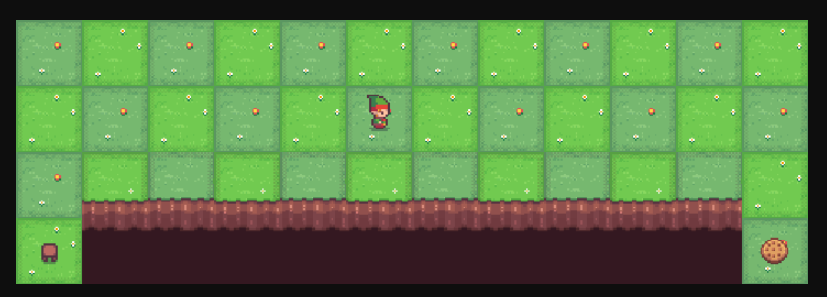
\includegraphics[width=0.8\linewidth]{figures/cliff_walking.png}
    \caption{El entorno Cliff Walking}
    \label{fig:cliff_walking_environment}
\end{figure}


\subsection{Estados, acciones y recompensas}
El entorno de Gymnasium contiene $4\times12=48$ posibles estados. De entre estos estados, solamente son posibles $3\times12+1=37$ estados, pues el agente puede estar en cualquiera de las celdas de las 3 filas superiores y, además, puede encontrarse en la casilla de salida. El agente no puede estar en ninguna de las celdas del acantilado ni en la celda de meta, pues esto ocasiona el final del episodio.

\subsubsection{Codificación del estado}
El estado del problema debe codificar la posición del gnomo en cada instante. Una solución obvia consistiría en definir el estado con las coordenadas $(i, j)$ de cada celda, recordando que en python ambas se numeran comenzado en 0. Sin embargo, resulta más conveniente codificar los estados con un único entero según se muestra en la figura \ref{fig:states}. Así pues, cuando el agente se encuentra en la posición $(i, j)$ del entorno, el estado entero se codifica como $s=i\times n_c+ j$, donde $n_c$ es el número de columnas del entorno (12). Por ejemplo, la posición de salida del agente se codifica con el entero 36 ($36 = 3\times 12+0$).

\begin{figure}
    \centering
    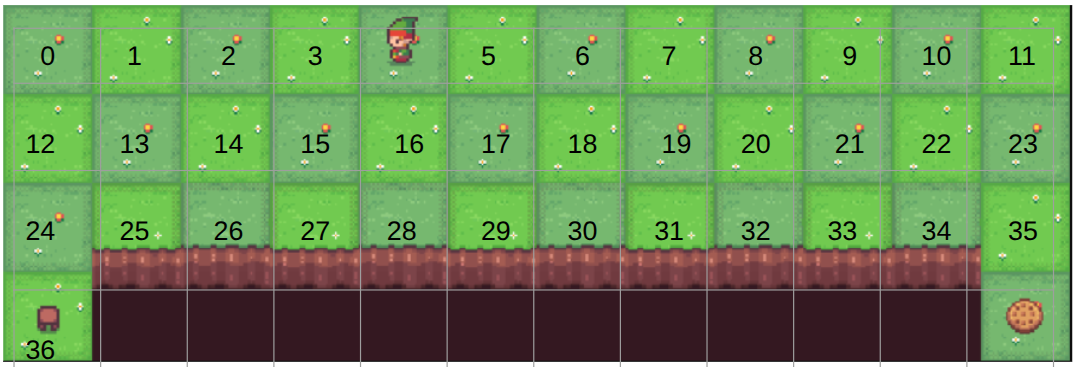
\includegraphics[width=0.8\linewidth]{figures/states.png}
    \caption{La codificación de estados del problema.}
    \label{fig:states}
\end{figure}


\subsubsection{Acciones}
En cada posición el agente puede realizar las siguientes acciones, codificada cada una de ellas con un número entero:
\begin{itemize}
    \item 0: arriba.
    \item 1: derecha.
    \item 2: abajo.
   \item  3: izquierda
\end{itemize}

\subsubsection{Recompensas}
El gnomo recibe una recompensa de -1 en cada paso del algoritmo. Se obtiene una recompensa de -100 cuando el agente se cae por el acantilado. Se desea que el gnomo alcance la meta con una suma de recompensas en el episodio máxima.


% \begin{exercise}
%     ¿Tendría sentido que se diera una recompensa mayor al agente cuando este se acerca al destino?
% \end{exercise}




\subsubsection{La tabla Q}
Con todo lo anterior, la tabla Q tiene la forma de esta matriz:
\begin{equation*}
    Q = \begin{bmatrix}
            q_{0,0} & q_{0,1} & q_{0,2} & q_{0,3}\\
            q_{1,0} & q_{1,1} & q_{1,2} & q_{1,3}\\
            \ldots & \ldots & \ldots & \ldots\\
            q_{36,0} & q_{36,1} & q_{36,2} & q_{36,3}\\
        \end{bmatrix}
\end{equation*}
La matriz tiene tantas filas como estados posibles se han codificado (48) y tantas columnas como posibles acciones a realizar en cada estado (4). Cada uno de los elementos $q_{i,j}$ almacena el valor de $Q(i, j)$ que estima las recompensas futuras que se obtendrían al realizar la acción $j$ cuando el agente se encuentra en el estado $i$. La técnica Q-learning propone una manera de estimar esta matriz para maximizar la recompensa de las acciones realizadas por el agente. En resumen: debemos calcular cada elemento de la matriz \texttt{q\_table} para que \texttt{q\_table[s][a]} estime la recompensa futura (sobre todos los estados
futuros hasta el final del episodio). La tabla \texttt{q\_table} la podemos encontrar si entramos en la clase \texttt{QLearning} (directorio \texttt{practice\_qlearning\_1/qlearning}):
\begin{verbatim}
    class QLearning():
    def __init__(self, environment, params):
        self.env = environment
        self.state_size = self.env.observation_space.n
        self.action_size = self.env.action_space.n
        self.q_table = np.zeros((self.state_size, self.action_size))
\end{verbatim}




\section{ACTIVIDADES I}

\subsection{Programación de un algoritmo de Q-learning}

% \begin{exercise}
%     Ejecute el script \texttt{practice\_q\_learning\_1/\\epsilon\_greedy\_tests.py}. Se abrirán tres gráficas consecutivamente. Observe la forma en la que decae el valor de $\epsilon$ en los tres casos comentados. Importante: fijaos en:
%     \begin{itemize}
%         \item La inicialización del objeto:
%         \begin{verbatim}
% epsilon_greedy_geom = EpsilonGreedyGeom(epsilon_max=1.0, 
%                                         epsilon_min=0.01,
%                                         total_episodes=1000,
%                                         percentage_target=0.25)   
%         \end{verbatim}        
%         \item La actualización de $\epsilon$:
%         \texttt{epsilon\_greedy\_geom.step()}
%     \end{itemize}
% \end{exercise}

% \begin{exercise}
%     ¿Cuál es la recompensa total de un episodio en el que el gnomo completa la tarea de forma óptima?
% \end{exercise}


%\subsubsection{Un primer script}

\begin{exercise}
Si abrimos el script \texttt{cliff\_q\_learning\_test.py}, encontraremos el siguiente script. Léalo con atención. 

\begin{verbatim}
from qlearning.qlearning import QLearning
import gymnasium as gym

def test_qlearning():
    environment = gym.make('CliffWalking-v1', render_mode="human")
    qlearning = QLearning(environment=environment)
    qlearning.create_random_q_table() 
    #qlearning.read_q_table(filename='qtable.npy')
    print('Testing mode!')
    qlearning.test(total_episodes_test=1)

if __name__ == "__main__":
    test_qlearning()
\end{verbatim}



La clase \texttt{QLearning} se proporciona programada \textbf{parcialmente}, para que el estudiante la complete. Importante:
\begin{itemize}
    \item En estos momentos la matriz Q no se conoce, con lo que el script genera una matriz Q aleatoria con el método \texttt{create\_random\_q\_table}.
    \item Si se utiliza la línea \texttt{qlearning.read\_q\_table(filename='qtable\_cliff.npy')} se cargará la tabla Q desde fichero. \textbf{Esto se deberá hacer cuando ya se haya entrenado y tengamos este fichero (script de train).}
    \item Si se ejecuta el script, el agente intentará resolver la tarea utilizando una matriz Q aleatoria: realizará movimientos de forma aleatoria sin llegar a su objetivo.
\end{itemize}\\
\textbf{EJERCICIO}\\
\begin{itemize}
    \item Ejecute el script \texttt{cliff\_q\_learning\_test.py}, al menos, 15 veces. Observe el comportamiento del agente. ¿Se consigue completar la tarea?    
    \item  ¿Cuál es la recompensa total de un episodio en el que el gnomo completa la tarea de forma óptima?
\end{itemize}

\end{exercise}


% Define a counter within sections




%\begin{exercise}
%Modifique el método \texttt{test} para calcular la %recompensa total de cada episodio $\sum_t=r_t$ y plotee el %resultado usando matplotlib.
%\end{exercise}

El Teorema del mono infinito afirma que un mono pulsando teclas al azar sobre un teclado durante un periodo de tiempo indefinido podrá escribir finalmente ``Hamlet'' de William Shakespeare (\url{https://es.wikipedia.org/wiki/Teorema_del_mono_infinito}). De la misma manera, podríamos generar tablas $Q$ aleatorias y pensar que alguna de ellas permitiría que el gnomo fuera desde la casilla de salida hasta la casilla de llegada. Si, por algún casual, ocurre esto (la probabilidad de que ocurra la trayectoria óptima es bastante fácil de calcular), este caso sería fácil de detectar y nos permitiría aproximar la tabla Q (pues cada valor de Q(i,j) tendría el valor total de recompensa del episodio). Sin embargo, la tabla Q calculada así dará difícilmente una solución óptima del problema: con mucha suerte el gnomo llegará a la casilla final... y con muchísima suerte la trayectoria realizada será óptima. También podríamos pensar qué hacer con diferentes tablas Q que resuelvan el problema de forma subóptima... para, de alguna manera intentar optimizarlo. La idea que se propone en esta práctica es diferente de la ``del mono''. Así pues, utilizaremos la ecuación de Bellman para actualizar los valores de Q en cada instante de simulación.

% \begin{exercise}
% \textbf{EJERCICIO\\}
%     Revise estas dos líneas en el script de test:
% \begin{verbatim}
%     qlearning.create_random_q_table()
%     #qlearning.read_q_table(filename=’qtable.npy’)
% \end{verbatim}
% La primera utiliza una tabla Q aleatoria. La segunda línea carga el valor de Q desde un fichero. Cuando se programe el script de entrenamiento, este calculará la matriz Q y la guardará en el fichero \texttt{qtable.npy}. Así pues, cuando tengamos una matriz Q calculada, tendremos que utilizar la segunda línea (\texttt{read\_q\_table}) para poder probar el resultado del entrenamiento.
% \end{exercise}

\begin{exercise}
\textbf{EJERCICIO}\\
Abra el fichero \texttt{practice\_qlearning\_1/qlearning/qlearning.py}. Busque la clase \texttt{QLearning()} y halle el método de test:
\begin{verbatim}
    def test(self, total_episodes):
\end{verbatim}
Examine el método test de la clase \texttt{QLearning}, y entienda su funcionamiento. \textbf{Ayuda}:
\begin{itemize}
    \item \texttt{state, info = self.env.reset()}: resetea el entorno a su estado inicial.
    \item \texttt{action = np.argmax(self.q\_table[state])}: la tabla se guarda en el array \texttt{self.q\_table}. Esta matriz tiene 48 filas y 4 columnas. Cada fila codifica un estado y cada columna una de las 4 acciones. \textbf{El valor máximo de cada fila} le indica al agente la acción más beneficiosa para maximizar las recompensas futuras. Así pues, la acción se calcula como el índice que corresponde con el máximo de los valores de la fila del estado actual, en python: \texttt{action = np.argmax(self.q\_table[state])}.
    \item Para ejecutar la acción sobre el entorno, se usa la función \texttt{step(action)}: \texttt{next\_state, reward, terminated, truncated, info = self.env.step(action)}
\end{itemize}
\end{exercise}

\begin{exercise}
\textbf{EJERCICIO}\\
%\subsection{Aprendizaje en el \textit{Cliff Walking environment}}
Abra el script \texttt{cliff\_q\_learning\_train.py}. Verá que el script es similar al script de \textit{test} vimos antes, con la diferencia de que en este caso guardamos la tabla Q al finalizar el método \emph{train}. La idea es la habitual en \textit{Machine Learning}: a) Entrenar y guardar Q. b) Testear: cargar Q y usarla para que el agente opere sobre el entorno. Se presenta el código, a continuación:
\begin{small}
\begin{verbatim}
def train_qlearning():    
    environment = gym.make('CliffWalking-v1', render_mode='human')
    qlearning = QLearning(environment=environment)
    print('LET US LEARN NOW!')
    qlearning.train(total_episodes_train=300)    
    qlearning.save_q_table(filename='qtable.npy')

if __name__ == "__main__":
    train_qlearning()    
\end{verbatim}
\end{small}

Use \texttt{render\_mode=human} si quiere ver la evolución del agente en el entorno. Normalmente, no haremos esto, pues ralentiza el aprendizaje:
\begin{verbatim}
    environment = gym.make('CliffWalking-v1', render_mode='human')
\end{verbatim}
Así pues, durante el aprendizaje, usaremos la siguiente configuración:
\begin{verbatim}    
    environment = gym.make('CliffWalking-v1')
\end{verbatim}
    





Si entramos en el método train (clase Qlearning), veremos esto:
\begin{small}
\begin{verbatim}
     def train(self, total_episodes_train):
        print("Training started!\n\n")

        raise NotImplementedError('EJERCICIO 6.3 sin completar': 
        debe completar QLearning.train()
        return self.q_table  
\end{verbatim}
\end{small}
    Complete el método \texttt{train} de la clase \texttt{QLearning}. \textbf{Nota}: deje el método \texttt{update\_q\_table} vacío (se completará en el apartado siguiente). Como ayuda se proporciona el pseudo código que permite entrenar y calcular la tabla Q. La mayoría de las funciones ya se han visto en el método de test anterior.
\begin{small}
\begin{verbatim}
    def train(self, total_episodes):
        epsilon_greedy = EpsilonGreedyGeom(...)
        - Repita durante un total de  total_episodes:
            - Resetee el entorno.
            while True: 
                
                - Tome una decisión de exploración o explotación: 
                (epsilon_greedy.random_action() devuelve True si hay que hacer una acción 
                aleatoria).
                
                - Aplique la acción sobre el entorno.
                next_state, reward, terminated, truncated, info = self.env.step(action)
            
                - Ejecute cada episodio hasta que terminated o truncated sea True.
                - Actualice la tabla Q con la ecuación de Bellman. Esto se programa en el
                método:
                self.update_q_table(state, action, next_state, reward)
               
                - Se actualiza la tabla Q con la nueva información:
                update_q_table(state, next_state, action, reward)
                
                - Pasamos al nuevo estado
                state = next_state
            # reducimos epsilon en cada episodio
            epsilon_greedy.step()
\end{verbatim}
\end{small}
\end{exercise}

Este pseudocódigo se puede resumir rápidamente: se simulan \texttt{total\_episodes} de entrenamiento. En cada episodio, se resetea el entorno a un estado inicial y se ejecutan una serie de pasos de simulación. El valor de $\epsilon$ y la forma en la que se reduce están definidos por la clase \texttt{EpsilonGreedyGeom}. Esta clase tiene una función \texttt{random\_action} que con probabilidad $\epsilon$ devuelve \texttt{True} (y se genera una acción aleatoria) y con probabilidad $1-\epsilon$ devuelve \texttt{False} y se obtiene la acción más adecuada de la tabla Q (según el valor de $Q(s,a)$ estimado hasta el momento). La clase \texttt{EpsilonGreedyGeom} se encarga de mantener el valor de epsilon y de actualizarlo (método \texttt{.step()}).  Cada acción se aplica sobre el agente y el entorno (\texttt{apply\_action}), lo que realiza la simulación instantánea del entorno y devuelve un nuevo estado y recompensa. Finalmente, se actualiza la tabla Q (ejercicio siguiente) con la función \texttt{update\_q\_table}. 

% \textcolor{red}{1. En clase yo había puesto otra formula para el decay de epsilon que contemplaba el valor máximo y aplicaba un exp, ver cuál de los dos utilizar. 2.La función apply action es la de self.env.step(action)?}
% \textcolor{blue}{He aclarado la fórmula que usa un decay rate. He visto que la usan mucho en otras librerías. La cuestión es que es fácil calcular el decay rate delta para que pase de epsilon max a epsilon min en un número de pasos. Lo he puesto en una clase \texttt{EpsilonGreedyGeom} que se encarga de mantener el valor de epsilon y de actualizarlo (\texttt{.step()}). He puesto una variación geométrica, lineal y time inverse. La exponenciaSi quieres, además de esa forma se puede programar el exponencial y el lineal}

% \textcolor{blue}{El pseudocódigo pretendía ser pseudocódigo... sin ser python, por eso las funciones no se llaman igual. Si ves que despista, lo pongo como algoritmo con el entorno algorithm de latex}



% \subsubsection{Actualización de Q (primera versión)}
% En esencia, la tabla $Q(s_t,a_t)=r_t$ se puede entender de la siguiente manera:
% \begin{itemize}
%     \item Dado un estado $s_t$.
%     \item Almacena un valor para cada una de las posibles acciones $a_t$ que puede ejecutar el agente en ese estado.
%     \item Sabemos que el agente elegirá la acción como: $a_t=argmax(Q(s_t, a_t))$.
% \end{itemize}

% Se propone una actualización de la tabla Q en la que se hace:
% $$Q(s_t,a_t)=r_t$$

\begin{exercise}
\textbf{EJERCICIO}\\
    Complete la función \texttt{update\_q\_table} usando la expresión de la Ecuación de Bellman:
    \begin{equation}
Q(s_t,a_t)_{i+1} = Q(s_t,a_t)_{i} + \alpha [r_t + \gamma 
\max_a(Q(s_{t+1},a))- Q(s_t,a_t)_{i}]  
\end{equation}
Se da aquí el prototipo:
    \begin{verbatim}
    def update_q_table(self, state, action, next_state, reward):
        self.q_table[state, action] = ...
    \end{verbatim}
    \textbf{Importante}: se ha definido una variable de la clase para almacenar la tabla Q: \texttt{self.q\_table}. También se han definido las variables de la clase \texttt{self.learning\_rate} ($\alpha$) y \texttt{self.discount} ($\gamma$).
\end{exercise}

\subsubsection{El ciclo de \textit{train-test}}
En estos momentos ya contamos con un algoritmo funcional para el aprendizaje. Una aplicación de aprendizaje automático se resume en los siguientes pasos:
\begin{itemize}
    \item[a)] Ejecutamos un entrenamiento durante un número de episodios: el código del script \texttt{cliff\_q\_learning\_train.py}. En este entrenamiento, usaremos un conjunto de hiperparámetros: $\alpha, \gamma, N$ y la estrategia de $\epsilon$.
    \item[b)] Evaluamos el resultado usando un script de test: \texttt{cliff\_q\_learning\_test.py}
    \item[c)] Si estamos satisfechos con el resultado del test $\Longrightarrow$ hemos terminado. Si estamos insatisfechos $\Longrightarrow$ \texttt{GOTO a)}.
\end{itemize}

Debemos darnos cuenta de:
\begin{itemize}
    \item Durante el entrenamiento se estima la matriz Q. Al final del entrenamiento esta matriz Q se guardará en el fichero \texttt{qtable.npy}. 
    \begin{verbatim}
        qlearning.save_q_table(filename=’qtable.npy’)
    \end{verbatim}
     \item Realizado el entrenamiento, se deberá probar la tabla Q para evaluar su conocimiento sobre la misión. El script de test deberá cargar la matriz Q desde el fichero \texttt{qtable.npy}. Así pues, se deberá modificar el script de test deberá hacer:
     \begin{verbatim}
        qlearning.read_q_table(filename='qtable.npy')
     \end{verbatim}
\end{itemize}


\begin{exercise}
\label{ej:alfa_gamma_cliff_walking}
\textbf{EJERCICIO}\\
Ejecute el algoritmo de entrenamiento durante 100 episodios (\texttt{cliff\_q\_learning\_train.py}). Use los parámetros: $\epsilon_0=1$, $N_{target}=0.25$ y $\epsilon_{min}=0.01$. Después:
\begin{itemize}
    \item[a)] Cambie los parámetros $\alpha$ y $\gamma$ de acuerdo con la tabla     \ref{tab:alfa_gamma_cliff_walking}. Puede hacer:
    \begin{verbatim}
        environment = gym.make(’CliffWalking-v1’, render_mode="human")
        params = {'alpha': 1.0, 'gamma': 0.99, 'percentage_target': 0.25}
        qlearning = QLearning(environment=environment, params=params)
    \end{verbatim}
    \item[b)] Para cada conjunto de parámetros, ejecute el script de \textit{train} y, a continuación, ejecute el script de \textit{test}. Observe el resultado.
    \item[c)] Complete los valores de la tabla \ref{tab:alfa_gamma_cliff_walking}: rellene la columna denominada ``ecuación'' y conteste sí/no, observando si el algoritmo aprende a resolver la tarea (evalúe el método de test y observe si el gnomo completa la misión).
\end{itemize}
\end{exercise}

\begin{table}[t]
\centering
\begin{tabular}{|c|c|c|c|}
\hline
 $\alpha$ & $\gamma$  & ``Ecuación de actualización''  & ¿Aprende?   \\\hline
 0 & 0 & 
$Q(s_t,a_t)_{i+1} = Q(s_t,a_t)_{i}$ & ¿?\\\hline
 0 & 1 & $Q(s_t,a_t)_{i+1} = Q(s_t,a_t)_{i}$ & ¿?\\\hline
1   & 0  &¿?  &¿?\\\hline
1& 1 & ¿? & ¿?\\\hline
0.5 & 0.99 & ¿? & ¿?\\\hline
\end{tabular}
\caption{Valores de $\alpha$ y $\gamma$ para el ejercicio \ref{ej:alfa_gamma_cliff_walking}.}
\label{tab:alfa_gamma_cliff_walking}
\end{table}

% \begin{exercise}
%     Ejecute el algoritmo de \textit{train} varias veces y responda a las siguientes cuestiones:
%     \begin{itemize}
%         \item ¿El algoritmo consigue aprender?
%         \item ¿El agente consigue completar la misión en algún momento?
%     \end{itemize}
% \end{exercise}


Según se ha podido comprobar, la función que permite actualizar los valores de la tabla Q depende de los valores de $\alpha$ y $\gamma$. Así pues, la ecuación de Bellman es una ``navaja suiza'' que se puede adaptar a la resolución de múltiples problemas de aprendizaje al variar $\alpha$ y $\gamma$. Sin embargo, es importante conocer cómo funcionan estos parámetros, pues hemos visto que es fácil caer en casos que no permiten obtener un aprendizaje eficaz. En consecuencia, es importante entender qué ocurre cuando se modifican los parámetros $\alpha$ y $\gamma$ de la ecuación de Bellman. En resumen, se ha comprobado que con $\alpha=0$ no se produce ningún aprendizaje, obviamente y que, también, la estrategia $Q(s_t, a_t)=r_t$ no produce, tampoco, ningún conocimiento (pues no propaga la información de otros estados ulteriores). Esta estrategia $Q(s_t,a_t)=r_t$ es \textbf{inadecuada}, pues está almacenando solamente la recompensa actual y no la suma de recompensas hasta el final. 






% \subsubsection{Actualización de Q (segunda versión)}
% Según se ha dicho, nos gustaría que $Q(s_t,a_t)$ guardara una estimación de las recompensas futuras que se obtendrían de estar en $s_t$ y tomar la acción $a_t$, es decir:
% $Q(s_t,a_t)=r_t + r_{t+1} + r_{t+2} + r_{t+3}$. Para ello, vamos a considerar que tenemos un entorno donde el número máximo de pasos es $T$ (como ocurre en la mayoría de entornos de Gymnasium). Así pues:
% \begin{equation}
% Q(s_t,a_t) = \sum_{i=t}^{T} r_i= r_t +  r_{t+1}+ \ldots + r_T
% \end{equation}
% Suponga que en el instante siguiente, la matriz también debería almacenar la suma de recompensas hasta el final del episodio:
% \begin{equation}
% Q(s_{t+1},a_{t+1}) = \sum_{i=t+1}^{T} r_i = r_{t+1} +r_{t+2} + \ldots + r_T     
% \end{equation}

% Podemos hacer: 
% \begin{equation}
%     Q(s_t,a_t) - Q(s_{t+1},a_{t+1}) = r_t
% \end{equation}
% Con lo que tenemos otra forma de actualizar la tabla Q:
% \begin{equation*}
% Q(s_t,a_t) = r_t + Q(s_{t+1},a_{t+1})   
% \end{equation*}

% Durante la simulación, en un instante determinado, conocemos que el agente está en $s_t$ y realiza la acción $a_t$. Como consecuencia, en ese mismo instante, el agente recibirá una recompensa $r_t$ (por ejemplo, si el agente se cae por el acantilado, $r_t=-100$. Si no se cae: $r_t=-1$). El problema ahora es que debemos sumar el término $Q(s_{t+1},a_{t+1})$. De este término, conocemos $s_{t+1}$ y tenemos 4 valores de Q (uno para cada acción posible). Con esto, ¿qué valor elegimos de $Q(s_{t+1},a_{t+1})$?. Esta parte se soluciona eligiendo el máximo de estos valores (). Así, se propone una \textbf{forma mejorada de la ecuación de actualización de la tabla Q}:
% \begin{equation*}
% Q(s_t,a_t) = r_t + max_a(Q(s_{t+1},a))
% \end{equation*}

% Nótese que esta ecuación se debe ejecutar de forma repetida para poder llegar a una estimación final, pues inicialmente se desconoce la tabla Q. 

% \subsubsection{El factor de descuento $\gamma$}
% En algunos entornos, la suma de recompensas siguiente no permite estimar correctamente la matriz. En la literatura se propone modificar la suma de recompensas:
% \begin{equation}
% Q(s_t,a_t) = \sum_t^{T} r_i= r_t +  r_{t+1}+ \ldots + r_T
% \end{equation}
% Por esta suma de recompensas:
% \begin{equation}
% Q(s_t,a_t) = r_t + \gamma r_{t+1}+ \gamma^2 r_{t+2} + \gamma^3r_{t+3} +  \ldots + \gamma^T r_T = \sum_{i=t}^{T} \gamma^{i-1}r_i
% \end{equation}
% Con este factor $0\leq\gamma\leq1$ se consigue que el agente pueda ponderar más las recompensas cercanas al instante $t$ (los pasos siguientes). Igual que hicimos antes:
% \begin{eqnarray*}
% Q(s_t,a_t) &=& r_t + \gamma r_{t+1}+ \gamma^2 r_{t+2} + \gamma^3r_{t+3} + \gamma^4r_{t+4} +  \ldots \\
% Q(s_{t+1},a_{t+1}) &=& r_{t+1} + \gamma r_{t+2}+ \gamma^2 r_{t+3} + \gamma^3r_{t+4} + \gamma^4r_{t+5} +  \ldots \\
% \end{eqnarray*}

% Aquí, vemos que se puede escribir:
% \begin{eqnarray*}
% Q(s_t,a_t) &=& r_t + \gamma 
% Q(s_{t+1},a_{t+1}) 
% \end{eqnarray*}
% E, igual que antes, nos deja la actualización siguiente de la tabla Q:
% \begin{eqnarray*}
% Q(s_t,a_t) &=& r_t + \gamma 
% \max_a(Q(s_{t+1},a))
% \end{eqnarray*}

% Obviamente, si ponemos $\gamma=1$, tenemos el caso en el que el agente suma todas las recompensas sin ponderar. Si ponemos, por ejemplo, $\gamma=0.5$, el agente considera solamente las recompensas cerca del instante actual y es bastante ``miope'' en relación con las recompensas futuras.

% \subsubsection{El factor de aprendizaje $\alpha$}
% Siempre que planteamos un proceso de aprendizaje, deberíamos plantear una forma de actualización del valor actual de un parámetro. Nótese que en la última ecuación se hacía:
% \begin{equation*}
% Q(s_t,a_t) = r_t + \gamma 
% max_a(Q(s_{t+1},a_{t+1}))
% \end{equation*}
% Con lo cual, el valor de $Q(s_t,a_t)$ se sustituye directamente con el nuevo valor $Q(s_t,a_t) = r_t + \gamma 
% \max_a(Q(s_{t+1},a_{t+1}))$. En el ámbito de la inteligencia artificial, generalmente se propone utilizar un factor de aprendizaje $\alpha$ que permite añadir más o menos información a la estimación actual en cada paso del algoritmo. Imaginemos que en la iteración $i$ tenemos una estimación $Q(s_t,a_t)_i$ de una celda de la tabla. La nueva estimación en la iteración siguiente es $Q(s_t,a_t)_{i+1}$. La nueva información de la que se dispone en el instante $i$ es $\hat{Q}(s_t,a_t) = r_t + \gamma 
% max_a(Q(s_{t+1},a_{t+1}))$:
% \begin{equation}
% \label{eq:learning_rate2}
% Q(s_t,a_t)_{i+1} = (1-\alpha) Q(s_t,a_t)_{i} + \alpha \hat{Q}(s_t,a_t)
% \end{equation}
% Con este parámetro $\alpha$ podemos regular la forma en la que se añade nuevo aprendizaje a la tabla Q. Así pues:
% \begin{itemize}
%     \item Si $\alpha=1$ el aprendizaje es máximo, y el algoritmo olvida la información anterior en cada instante de simulación.
%     \item Si $\alpha=0$ el aprendizaje es mínimo y no se añade nueva información a la tabla Q.
% \end{itemize}

% \section{La ecuación de Bellman}
% Con todo lo anterior, escribimos la ecuación de actualización completa sustituyendo en la ecuación (\ref{eq:learning_rate2}) el valor de actualización propuesto $\hat{Q}(s_t,a_t) = r_t + \gamma 
% \max_a(Q(s_{t+1},a_{t+1}))$. Quedando:
% \begin{equation}
% Q(s_t,a_t)_{i+1} = Q(s_t,a_t)_{i} + \alpha [r_t + \gamma 
% \max_a(Q(s_{t+1},a))- Q(s_t,a_t)_{i}]    
% \end{equation}

% Así pues, esta última ecuación se conoce como la Ecuación de Bellman. El matemático Richard Ernest Bellman la propuso en los años 50. La ecuación nos deja dos parámetros muy interesantes ($\alpha$ y $\gamma$) que podemos variar para resolver diferentes problemas de Q-learning.

% Así pues, en resumen, tenemos los siguientes parámetros

\section{Resumen}
El código siguiente permite resolver un problema de aprendizaje e incluye todos los conceptos que hemos visto hasta ahora:
\begin{verbatim}
    def train(self, total_episodes):
        self.results = []
        print('Training started!', flush=True)
        epsilon_greedy = EpsilonGreedyGeom(epsilon_max=self.epsilon_max,
                                       epsilon_min=self.epsilon_min,
                                       total_episodes=total_episodes,
                                       percentage_target=self.percentage_target)
        recent_rewards = []
        for episode in range(total_episodes):
            state, info = self.env.reset()
            total_reward = 0
            while True:
                if epsilon_greedy.random_action():
                    action = self.env.action_space.sample()  # Explore
                else:
                    action = np.argmax(self.q_table[state])  # Exploit
                next_state, reward, terminated, truncated, info = self.env.step(action)
                total_reward += reward
                self.update_q_table(state, action, next_state, reward)
                if terminated or truncated:
                    break
                state = next_state
            epsilon_greedy.step()
        print("Training finished! Your Q-table is optimized.")
        return self.q_table

    def update_q_table(self, state, action, next_state, reward):
        # Update Q-table using the Bellman Equation
         self.q_table[state, action] = (self.q_table[state, action] +
                    self.learning_rate * (reward + self.discount_rate * 
                    np.max(self.q_table[next_state]) -
                    self.q_table[state, action]))

    def test(self, total_episodes, save_results=False):
        recent_rewards = []
        for episode in range(total_episodes):
            state, info = self.env.reset()
            total_reward = 0
            while True:
                action = np.argmax(self.q_table[state])  
                next_state, reward, terminated, truncated, info = self.env.step(action)
                total_reward += reward
                if self.env.render_mode == 'human':
                    time.sleep(.1)
                if terminated or truncated:
                    break
                state = next_state
            recent_rewards.append(total_reward)
            if save_results:
                self.results.append([episode, total_reward, 0])
            print(f"Episode {episode:4d} | Total reward: {total_reward:6.1f}", end='\r')
            if episode % 10 == 0:
                print()
        return recent_rewards
\end{verbatim}
%En resumen, hemos visto cómo actualizar la tabla de acuerdo con la ecuación de Bellman. 
%\begin{equation}
%Q(s_t,a_t)_{i+1} = Q(s_t,a_t)_{i} + \alpha [r_t + \gamma 
%\max_a(Q(s_{t+1},a))- Q(s_t,a_t)_{i}]    
%\end{equation}






\section{Otro entorno más desafiante: Taxi v3}
En este entorno existe un taxi que puede moverse por el mapa que simula una ciudad (figura \ref{fig:taxi}). La misión consiste en recoger a un pasajero de una posición determinada para dejarlo en el hotel. Tanto la posición de recogida como la de destino pueden variar en cada simulación.

En este problema, a diferencia del entorno \textit{Cliff Walking}, los estados iniciales serán diferentes. Esto incluye variaciones de la posición inicial del taxi, de la posición inicial del pasajero y del destino. Se excluyen de estos estados iniciales (la librería gymnasium los elimina automáticamente) los casos ilegales en los que el pasajero ya se encuentra dentro del vehículo, o si el vehículo y el pasajero se encuentran ya en el destino.
\subsection{Descripción del entorno}
\subsubsection{Acciones}
El taxi puede realizar las siguientes acciones:
\begin{itemize}
    \item 0: Move south (down).
    \item 1: Move north (up).
    \item 2: Move east (right).
    \item 3: Move west (left).
    \item 4: recoger al pasajero.
    \item 5: dejar al pasajero.
\end{itemize}

\subsubsection{Estado}
El estado de este problema debe codificar:
\begin{itemize}
    \item La posición del taxi en una rejilla de $5\times 5$.
    \item La posición del pasajero: 
    \begin{itemize}
        \item 0: Red
        \item 1: Green
        \item 2: Yellow
        \item 3: Blue
        \item 4: In taxi
    \end{itemize}
    \item Los posibles destinos del pasajero (la posición del hotel): 
    \begin{itemize}
        \item 0: Red
        \item 1: Green
        \item 2: Yellow
        \item 3: Blue
    \end{itemize}
\end{itemize}

Con todo esto, hay 500 estados posibles, pues existen:
\begin{itemize}
    \item 25 posiciones posibles en las que se encuentra el taxi.
    \item Hay 5 posiciones posibles para el pasajero (4 cuadros de colores y, además, el caso en el que el pasajero está montado en el coche).
    \item Finalmente, hay 4 destinos posibles para el pasajero.
\end{itemize}
En total son $n_s=25\times5\times4$ estados posibles. El estado se codifica como un entero que se calcula como: 

\texttt{state=((taxi\_row * 5 + taxi\_col) * 5 + passenger\_location) * 4 + destination}

No obstante, de entre todos los estados anteriores, solamente hay 404 que pueden ser alcanzados en un episodio. Los estados que faltan corresponden con situaciones en las que el pasajero se encuentra ya en la misma posición de destino (pues en ese momento, el episodio acaba). El caso en el que el taxi y el pasajero están en la misma casilla de destino puede observarse justo después de que el episodio acabe.

\subsubsection{Estado inicial}
El estado inicial se genera de forma aleatoria de entre los estados válidos donde el pasajero no se encuentra ya en el destino ni dentro del taxi. En total, existen 300 estados iniciales diferentes.

\subsubsection{Recompensas}
En el caso del taxi, las recompensas se definen así:
\begin{itemize}
    \item -1 por cada paso, si no se obtiene otra recompensa.
    \item +20 por dejar al pasajero en el destino (correcto).
    \item -10 por recoger o dejar al pasajero de forma ``ilegal''.
\end{itemize}

Así pues, el hecho de realizar un paso (step) conlleva una recompensa negativa, pues buscamos que el taxi realice el transporte del pasajero de inicio a final en el mínimo tiempo posible (se desea maximizar la suma de recompensas recibidas). Cuando se deja al pasajero, se obtiene una recompensa positiva (+20). Nótese que se obtiene una recompensa negativa por acciones ilegales de recogida y reparto de la persona: pues podría ocurrir que el agente decidiera dejar al pasajero lejos de su destino o bien intentar recogerlo en una casilla donde no estuviera la persona).

Un acción que conlleve que el Taxi no se mueva, como, por ejemplo, intentar ir contra un obstáculo, incurre en una recompensa negativa (-1). 

\subsubsection{Final del episodio}
El episodio acaba cuando el taxi deja al pasajero en la posición adecuada (\texttt{terminated=True}). El episodio acaba cuando la duración del episodio excede los 200 pasos (\texttt{truncated=True}).

\begin{figure}
    \centering    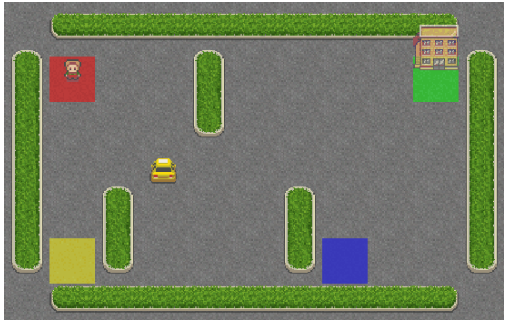
\includegraphics[width=0.8\linewidth]{figures/taxi.png}
    \caption{El entorno Taxi.}
    \label{fig:taxi}
\end{figure}

\subsection{ACTIVIDADES II}
Los ficheros de esta parte de la práctica son:
\begin{itemize}
    \item Entrenamiento: \texttt{taxi\_q\_learning\_train.py}.
    \item Test: \texttt{taxi\_q\_learning\_test.py}.
\end{itemize}

Si prestamos un segundo de atención a la clase QLearning que habéis programado, vemos lo siguiente:
\begin{verbatim}
    class QLearning():
    def __init__(self, environment, params):
        self.env = environment        
        self.state_size = self.env.observation_space.n
        self.action_size = self.env.action_space.n     
        self.q_table = np.zeros((self.state_size, self.action_size))
        self.learning_rate = params.get('alpha', 1.0)  # alpha
        self.discount_rate = params.get('alpha', 0.9)  # gamma
        self.percentage_target = 0.25
        self.max_epsilon = params.get('max_epsilon', 1.0)
        self.min_epsilon = params.get('min_epsilon', 0.01)        
\end{verbatim}

En efecto, cuando creamos un objeto de la clase \texttt{QLearning}, la tabla Q se inicializa automáticamente consultando el tamaño del estado y de las acciones con el entorno que le pasamos (\texttt{environment}). Así pues, el mismo código que hemos usado para resolver el entorno \textit{Cliff Walking} lo podemos usar para el problema del Taxi y para cualquier otro problema de Q-learning en el que podamos describir el estado de forma discreta. En la parte final del método \texttt{\_\_init\_\_} se guardan los parámetros que hemos comentado anteriormente: $\alpha$, $\gamma$ y la estrategia $\epsilon$-greedy que definen los parámetros de la Ecuación de Bellman y la forma de hacer la exploración/explotación de Q durante el entrenamiento. Para poder modificar estos parámetros, en la clase habrás visto que se hace \texttt{self.min\_epsilon = params.get('min\_epsilon', 0.01)}: esta parte del código busca un parámetro en el diccionario y, si no se encuentra, guarda un valor por defecto.

En esencia, podemos entrenar el entorno del taxi directamente y solamente nos debemos preocupar de seleccionar unos parámetros $\alpha$, $\gamma$, $\epsilon_{max}$, $\epsilon_{min}$ y $N_{target}$ (\texttt{self.percentage\_target}) que permitan optimizar el aprendizaje del agente. En el apartado siguiente experimentaremos con diferentes valores de estos parámetros y observaremos los resultados.


\subsection{¿Está aprendiendo el agente?}
Comenzamos ejecutando directamente el script de entrenamiento unos hiperparámetros para los que pensamos que funcionará el aprendizaje.

\begin{exercise}
\textbf{EJERCICIO}\\
    Ejecute el script de entrenamiento \texttt{taxi\_q\_learning\_train.py} con 300 episodios de entrenamiento y los siguientes valores de \textit{learning rate} y \textit{discount rate}: $\alpha=0.1$, $\gamma=0.5$. 
\begin{verbatim}
def train_qlearning():
    environment = gym.make('Taxi-v3')
    params = {'alpha': 1.0, 'gamma': 1.0}
    qlearning = QLearning(environment=environment, params=params)
    qlearning.train(total_episodes=300)
    qlearning.save_q_table(filename='qtable_taxi.npy')
    
if __name__ == "__main__":
    train_qlearning()    
\end{verbatim}
Ejecute, después, el script de test \texttt{taxi\_q\_learning\_test.py}. ¿Se consigue completar la misión? ¿Ha aprendido el agente?
\end{exercise}

Vemos que el problema del taxi, es más complejo que el problema del acantilado, pues hay un mayor número de estados y acciones posibles. En consecuencia, previsiblemente, se necesitará un mayor número de episodios de entrenamiento para que se produzca un aprendizaje significativo. En el ejercicio anterior (salvo que hayamos sido muy afortunados) no se consigue resolver la tarea correctamente. Como no se ha producido un buen aprendizaje, nos preguntamos:
\begin{itemize}
    \item ¿Debemos aumentar el número de episodios para el entrenamiento?
    \item ¿O debemos cambiar los valores de los parámetros $\gamma$ y $\alpha$?    
    \item ¿Debemos cambiar la estrategia $\epsilon$-greedy?    
\end{itemize}




 Efectivamente, es necesario saber qué esta pasando en cada episodio durante el entrenamiento. En caso contrario, iremos ``a ciegas''. Cuando nos enfrentamos a problemas de aprendizaje más complejos, \textbf{es vital que sepamos si se está produciendo algún tipo de aprendizaje, pues durante el entrenamiento se está utilizando tiempo de cómputo y energía (ambos valiosos)}. En caso de que sospechemos que no se esté obteniendo un buen aprendizaje, deberíamos parar el entrenamiento y volver a la fase de diseño. Hay diferentes formas de evaluar el aprendizaje durante la fase de entrenamiento. Una forma sencilla es la siguiente: en un porcentaje de episodios de entrenamiento (por ejemplo, en uno de cada 10), se desactiva la opción $\epsilon$-greedy y se toman todas las acciones del episodio en base a la tabla Q (se evitan las acciones aleatorias). Mientras se hace eso, se calcula la recompensa total del episodio.



 
\begin{exercise}
\textbf{EJERCICIO}\\
Se desea medir el aprendizaje durante los diferentes episodios de entrenamiento. Para ello, es necesario modificar el método de entrenamiento (según se ha explicado anteriormente). Partiendo del script \texttt{taxi\_q\_learning\_train.py}: 
\begin{itemize}
    \item Modifique el método de train de la clase \texttt{QLearning}.
    \item Cree una método denominado \texttt{self.inline\_test()} en la clase \texttt{QLearning}. 
    \item En el método de train, cada 10 episodios de entrenamiento el método \texttt{self.inline\_test()} deberá ejecutar 10 episodios de test. La función debe devolver \textbf{la recompensa media de esos 10 episodios}, pues el resultado de cada test puede ser diferente.
    \item En cada test \textit{inline}, solamente se explota el conocimiento inherente a Q (no se toman acciones aleatorias).
    \item En el método train se debe guardar el resultado de cada llamada a \texttt{self.inline\_test()}. Se debe devolver la lista.
     \item Plotee los resultados al finalizar el entrenamiento.
\end{itemize}
Haga:
\begin{itemize}
    \item Un entrenamiento con $\alpha=0.9$ y $\gamma=0.1$ de 1500 episodios (habrá 150 episodios de test).
    \item Un entrenamiento con $\alpha=0.5$ y $\gamma=0.5$ de 1500 episodios (habrá 150 episodios de test).    
    \item Las combinaciones cruzadas de parámetros que faltan.
\end{itemize}
\begin{verbatim}
def train_qlearning():
    environment = gym.make('Taxi-v4')
    params = {'alpha': 0.5, 'gamma': 1.0}
    qlearning = QLearning(environment=environment, params=params)
    results = qlearning.train(total_episodes=1500)
    qlearning.save_q_table(filename='qtable_taxi.npy')
    plt.figure()
    plt.plot(results)
    plt.ylabel('Mean reward')
    plt.xlabel('Episodes (inline tests)')
    plt.show()
\end{verbatim}
%Compare las dos gráficas con matplotlib. 
%Toda la funcionalidad para representar los experimentos la encontrarás en el script \texttt{taxi\_q\_learning\_train\_graphs.py}. Tendrás únicamente que modificar el método \texttt{train} de la clase \texttt{QLearning()} para guardar la recompensa total en los episodios que exploten Q.
\end{exercise}

Se muestra en la figura \ref{fig:inline_tests_0.5_1.0} el resultado Un resultado típico de un entrenamiento de 2000 episodios con $\alpha=0.5$ y $\gamma=1.0$, usando una función de $\epsilon$ geométrica 25/75. Vemos cómo aumenta la recompensa media (medido con un \textit{inline test}). Hacia los episodios finales la recompensa media se estabiliza, acabando en valores positivos que resuelven el problema del entorno Taxi. Un resultado peor se obtiene con $\alpha=0.1$ y $\gamma=1.0$ (figura \ref{fig:inline_tests_0.1_1.0}).

\begin{figure}
    \centering
    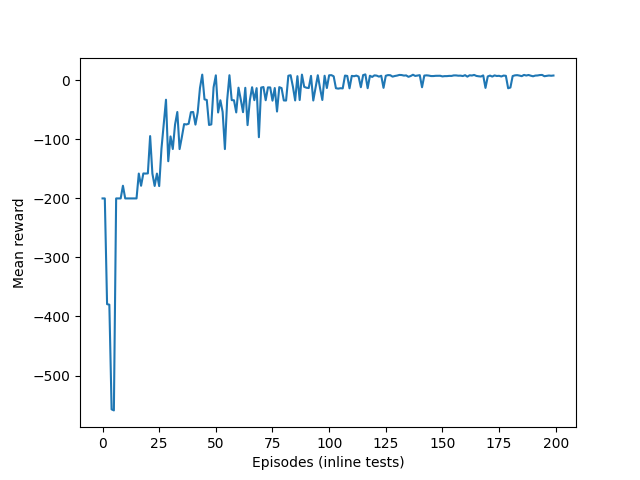
\includegraphics[width=0.8\linewidth]{figures/inline_test_alpha_0.5_gamma_1.0.png}
    \caption{Recompensa media durante el entrenamiento con $\alpha=0.5$ y $\gamma=1.0$.}
    \label{fig:inline_tests_0.5_1.0}
\end{figure}
\begin{figure}
    \centering
    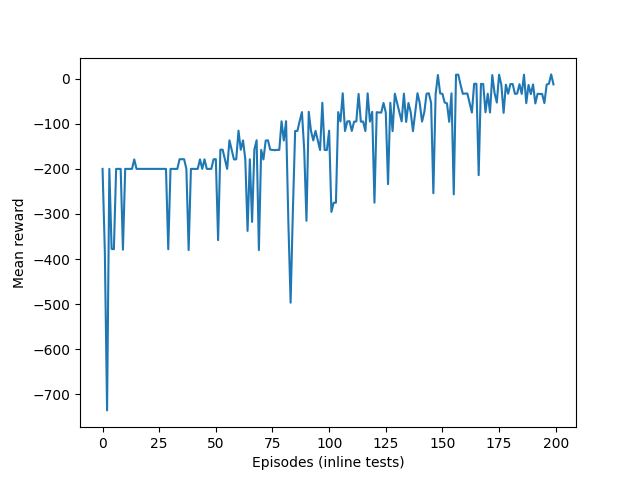
\includegraphics[width=0.8\linewidth]{figures/inline_test_alpha_0.1_gamma_1.0.png}
    \caption{Recompensa media durante el entrenamiento con $\alpha=0.1$ y $\gamma=1.0$.}
    \label{fig:inline_tests_0.1_1.0}
\end{figure}

Hecha la prueba anterior, posiblemente, no tengamos muy claro cuáles son los parámetros que permiten obtener un mejor aprendizaje del entorno. En general, los valores óptimos de los hiperparámetros dependen fuertemente del entorno. Una forma de hallar los parámetros óptimos para un entorno es realizar varios entrenamientos diferentes del entorno con todas las combinaciones de $\alpha$ y $\gamma$. 

%En la figura \ref{fig:figure_alpha_gamma} se muestra la recompensa total de los episodios de test intermedios para diferentes combinaciones de $\alpha$ y $\gamma$. Es importante darse cuenta de que con algunas combinaciones de $\alpha$ y $\gamma$ el agente no llega a aprender correctamente nunca. Por ejemplo, la combinación $(\alpha, \gamma)=(0.1, 0.1)$ es desastrosa. Aparentemente la configuración $(\alpha, \gamma)=(0.1, 0.9)$ tarda más episodios en aprender que el resto. Finalmente, la mejor combinación parece ser la $(\alpha, \gamma)=(0.5, 0.9)$, que aprende más rápido que la $(\alpha, \gamma)=(0.5, 0.1)$, ambas llegando a valores de recompensa total similares. Nos damos cuenta de que esta gráfica es \textbf{complicada de visualizar cuando tenemos muchos combinaciones diferentes}. Resultaría interesante realizar entrenamientos de 500 episodios y calcular la recompensa media de cada episodio de test intermedio.

\begin{exercise}
\textbf{EJERCICIO}
Abra el script \texttt{taxi\_q\_learning\_train\_opt.py}. Observe que aquí se plantea algo diferente: 
\begin{itemize}
    \item Se realiza un entrenamiento con diferentes valores de $\alpha$ y $\gamma$.
    \item Se testea el resultado durante un buen número de episodios y se guarda el resultado medio en un array bidimensional.
\end{itemize}

Realice lo siguiente:
\begin{itemize}
    \item Utilice \texttt{np.linspace(0.05, 1, 5)} para hallar 5 valores de $\alpha$ y $\gamma$ en el intervalo $[0.05, 1]$.
    \item Modifique \texttt{total\_epidodes\_train = 1500, total\_epidodes\_test = 500}.
    \item Observe el mapa de calor resultante.
\end{itemize}
\textbf{Nota}: se está haciendo un barrido con ``fuerza bruta'' de todos los posibles valores de parámetros, con lo que es normal que el script tarde bastante en ejecutarse.\\
\textbf{Nota}: se han probado 25 combinaciones diferentes de parámetros. Si quisiéramos ``afinar'' más el resultado, podríamos hacer, por ejemplo \texttt{np.linspace(0.5, 1, 15)} en ambos parámetros, pues ya hemos podido descartar algunas combinaciones que no producen buenos resultados.
\end{exercise}

Deberías obtener un resultado como el de la figura \ref{fig:figure_alpha_gamma_heatmap}. Se muestra un mapa de calor donde tenemos varios puntos de $\alpha$ y $\gamma$ con valores de aprendizaje similares. Deberíamos aumentar el número de episodios de \textit{train} y \textit{test} para poder encontrar diferencias significativas (incrementando enormemente el tiempo de cómputo total). En base a los resultados, vemos que podemos obtener buenos valores de aprendizaje con $\alpha \in [0.4, 0.9]$ y $\gamma=1.0$.
%Nótese que el proceso es muy ruidoso, con lo que debemos utilizar un número alto de episodios de entrenamiento. También usamos un número alto de episodios de test para probar concienzudamente el resultado. 
%i ejecutamos dos veces el entrenamiento con los mismos valores de $\alpha$ y $\gamma$, no obtendremos el mismo valor medio. Para reducir el error en esta medida, se puede repetir el episodio varias veces con los mismos valores de $\alpha$ y $\gamma$. Esto, obviamente, aumenta mucho el tiempo para hacer estos cálculos. 
%Finalmente, y volviendo a la figura \ref{fig:figure_alpha_gamma_heatmap}, sería conveniente repetir el experimento con más valores.



%\begin{figure}
%    \centering    \includegraphics[width=0.8\linewidth]{figures/Figure_alpha_gamma.png}
%    \caption{Aprendizaje en cada episodio del  entorno Taxi con diferentes valores de $\alpha$ y $\gamma$.}
%    \label{fig:figure_alpha_gamma}
%\end{figure}


\begin{figure}
    \centering    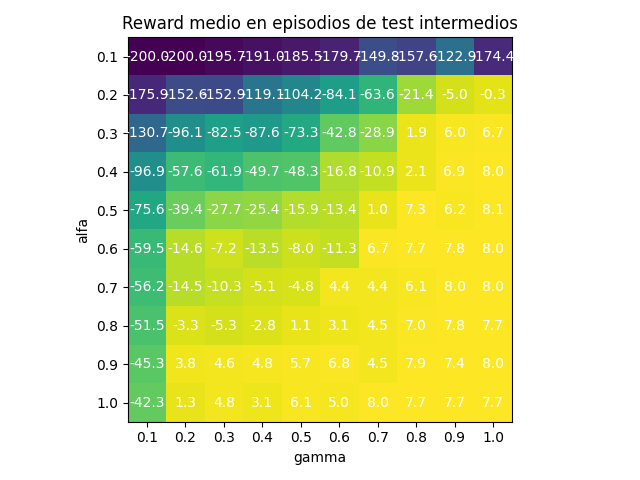
\includegraphics[width=0.8\linewidth]{figures/Figure_alpha_gamma_heatmap.png}
    \caption{Aprendizaje medio de diferentes combinaciones de $\alpha$ y $\gamma$ en episodios de test intermedios. Entorno: Taxi.}
    \label{fig:figure_alpha_gamma_heatmap}
\end{figure}

%\section{ACTIVIDADES II}




\section{Instalación}
Los equipos de prácticas tienen todo lo necesario para realizar la práctica. En este apartado se dan algunas instrucciones para que puedas instalar todo lo necesario en otro portátil/PC y poder trabajar de forma autónoma en tu propio PC/portátil. Las instrucciones se ofrecen para un sistema Linux/Ubuntu. 
Comenzamos instalando el programa git:
\begin{verbatim}
$ sudo apt install git
\end{verbatim}

Comenzamos por descargarnos el repositorio de prácticas. Es un repositorio que se encuentra en Github:
\begin{verbatim}
$ cd /home/usuario/Desktop
$ git clone https://github.com/4rtur1t0/Intro2AI
\end{verbatim}
Veremos que tenemos un directorio llamado Intro2AI en el escritorio. Seguimos instalando algunos paquetes necesarios para la creación de entornos virtuales de python \texttt{virtualenv}:
\begin{verbatim}
sudo apt install python3-pip python3-venv python3-dev -y 
\end{verbatim}

Seguidamente, creamos un entorno virtual:
\begin{verbatim}
$ cd /home/usuario
$ mkdir Applications
$ cd Applications
$ virtualenv venvAI
$ source /home/usuario/Applications/venvAI/bin/activate
\end{verbatim}
Con esto hemos creado un entorno virtual de python en el directorio \texttt{/home/usuario/Applications/venvAI} y lo hemos activado. Instalamos ahora algunos paquetes para este entorno de python:
\begin{verbatim}
$ cd /home/usuario/Applications/venvAI/bin
$ sudo apt install swig
$ ./pip install -r /home/arturo/Desktop/Intro2AI/requirements.txt 
$ ./pip install stable-baselines3 swig torch
$ ./pip install tensorboard
$ ./pip install "gymnasium[atari,accept-rom-license]" stable-baselines3 shimmy
\end{verbatim}

Cuando usemos un editor de python, como, pyCharm o Visual Studio, necesitaremos asociar el entorno virtual que hemos creado con el proyecto.

% import gymnasium as gym
% import numpy as np
% import random

% # Initialize environment
% env = gym.make("Taxi-v3")

% # Initialize Q-table with zeros (500 states x 6 actions)
% state_size = env.observation_space.n
% action_size = env.action_space.n
% q_table = np.zeros((state_size, action_size))

% # Hyperparameters
% total_episodes = 2000
% learning_rate = 0.1      # alpha
% discount_rate = 0.6      # gamma
% epsilon = 1.0            # Exploration rate
% max_epsilon = 1.0
% min_epsilon = 0.01
% decay_rate = 0.01        # Exponential decay rate for exploration

% # Training loop
% for episode in range(total_episodes):
%     state, info = env.reset()
%     done = False
    
%     while not done:
%         # Step 1: Epsilon-greedy action selection
%         if random.uniform(0, 1) < epsilon:
%             action = env.action_space.sample() # Explore
%         else:
%             action = np.argmax(q_table[state]) # Exploit
            
%         # Step 2: Take action, observe new state and reward
%         next_state, reward, terminated, truncated, info = env.step(action)
%         done = terminated or truncated
        
%         # Step 3: Update Q-table using the Bellman Equation
%         q_table[state, action] = q_table[state, action] + learning_rate * (
%             reward + discount_rate * np.max(q_table[next_state]) - q_table[state, action]
%         )
        
%         # Move to next state
%         state = next_state
        
%     # Reduce epsilon (less exploration, more exploitation as time goes on)
%     epsilon = min_epsilon + (max_epsilon - min_epsilon) * np.exp(-decay_rate * episode)

% print("Training finished! Your Q-table is optimized.")
% env.close()


% Cuestiones que se pueden preguntar:
% Variaciones sobre estos parámetros. ¿En qué afectan? → a la memoria de prácticas.
% total_episodes = 2000
% learning_rate = 0.1      # alpha
% discount_rate = 0.6      # gamma
% epsilon = 1.0            # Exploration rate
% max_epsilon = 1.0
% min_epsilon = 0.01
% decay_rate = 0.01    
% ¿qué pasa cuando variamos el decay rate? ¿qué se observa? ¿qué pasa si se hace una función lineal o exponencial?

% La solución es óptima (la trayectoria es óptima).

% Suponga que el pasajero está a bordo. Para todos los estados (todas las casillas).
% Haga un mapa que muestre el valor de la acción SOUTH sobre todas las casillas
% Haga un mapa que muestre el valor de la acción WEST sobre todas las casillas
% Haga un mapa que muestre el valor de la acción SOUTH-WEST sobre todas las casillas.


% Podemos seguir aprendiendo mientras se opera en modo funcionamiento. En nuestro problema del taxi se opera en una ciudad. Imagine un taxista experimentado que trabaja en Madrid. Un buen día (o malo) le cortan la castellana (una de las casillas ). ¿Puede el taxista aprender esta situación?



% ¿FUNCIONA?
% Pues en efecto, se os proporciona poco código y estamos luchando para que lo escribáis vosotros mismos.
% Pues le puedes preguntar a la IA si funciona tu código, aquí tienes una probabilidad de que te dé una versión probada del algoritmo de los muchos repositorios que hay por internet de gente que ha encontrado soluciones.
% El objetivo es que tú aprendas a encontrar estas soluciones y a encontrar


% EJERCICIO
% Nos gustaría poder analizar el reward de cada episodio, para las acciones que se tomen de acuerdo con el conocimiento de la tabla… y no las que se tomen aleatoriamente. →

% Podríamos forzar algún episodio durante el entrenamiento con epsilon nulo, para evaluar el desempeño.

% EJERCICIO
% Evalúe el entrenamiento en base a la recompensa media.







\bibliographystyle{alpha}
\bibliography{sample}

\end{document}
